\documentclass[thesis=M,czech]{FITthesis}[2011/06/14]

\usepackage[utf8]{inputenc} % LaTeX source encoded as UTF-8
\usepackage{textcomp}
\setcounter{tocdepth}{2}

\usepackage{graphicx} %graphics files inclusion
% \usepackage{amsmath} %advanced maths
% \usepackage{amssymb} %additional math symbols

\usepackage[acronym,nonumberlist,toc,sanitize={name=false,description=false},xindy={language=czech,codepage=utf8,glsnumbers=false}]{glossaries}
\addto\captionsczech{\renewcommand\acronymname{Seznam pou{\v z}it{\' y}ch zkratek}}
\addto\captionsczech{\renewcommand\glossaryname{Glosář}}
\deftranslation[to=czech]{Acronyms}{Seznam pou{\v z}it{\' y}ch zkratek}
\deftranslation[to=czech]{Glossary}{Glosář}

\newcommand{\tg}{\mathop{\mathrm{tg}}} %cesky tangens
\newcommand{\cotg}{\mathop{\mathrm{cotg}}} %cesky cotangens

% % % % % % % % % % % % % % % % % % % % % % % % % % % % % % 
% ODTUD DAL VSE ZMENTE
% % % % % % % % % % % % % % % % % % % % % % % % % % % % % % 

% http://www.ctan.org/tex-archive/macros/latex/contrib/fixme/
% \usepackage{xkvltxp}
% \usepackage[footnote,draft,silent,nomargin]{fixme}

\definecolor{poznamka}{rgb}{1.0,0.7,0.0}
\newglossary[tlg]{todo}{tdo}{tdu}{Seznam úkolů}
\newcounter{todo}
\newcommand{\todo}[1]{{{\newglossaryentry{\arabic{todo}}{type=todo,name={\arabic{todo}},description={#1},sort={#1}}} {\color{poznamka} \textbf{TODO} \glsdesc{\arabic{todo}}} {\stepcounter{todo}}}}
% \newcommand{\todo}[1]{{\color{poznamka}{TODO #1}}}
\newcommand{\mytitle}{Průvodce studenta FIT ČVUT}
\newcommand{\myauthor}{Jan Molnár}

\department{Katedra softwarového inženýrství}
\title{\mytitle}
\author{\myauthor} %jméno autora bez akademických titulů
\authorWithDegrees{Bc. Jan Molnár} %jméno autora včetně akademických titulů
\supervisor{Ing. Michal Havryluk}
\acknowledgements{Doplňte, máte-li komu a za co děkovat. V~opačném případě úplně odstraňte tento příkaz.}% Ing. Havryluk, doc. Vitvar, Týna, rodiče, autoři knihoven, autoři použitých FS aplikací, autoři myšlenek svobodného SW...
\abstractCS{V~několika větách shrňte obsah a přínos této práce v~češtině. Po přečtení abstraktu by se čtenář měl mít čtenář dost informací pro rozhodnutí, zda chce Vaši práci číst.}
\abstractEN{Sem doplňte ekvivalent abstraktu Vaší práce v~angličtině.}
\placeForDeclarationOfAuthenticity{V~Praze}
\keywordsCS{Nahraďte seznamem klíčových slov v češtině oddělených čárkou.}
\keywordsEN{Nahraďte seznamem klíčových slov v angličtině oddělených čárkou.}


\hypersetup{pdftitle={\mytitle},pdfauthor={\myauthor}}
\makeglossaries
\begin{document}
% \selectlanguage{czech}
% Nutné ve zkratkách převádět písmena kvůli řazení Č -> {\v C}!
\newacronym{AIISO}{AIISO}{Academic Institution Internal Structure Ontology}
\newacronym{BSD}{BSD}{Berkeley Software Distribution} 
\newacronym{CD}{CD}{Compact Disc}
\newacronym{CSS}{CSS}{Cascading Style Sheets}
\newacronym{CVUT}{{\v C}VUT}{České vysoké učení technické v Praze}
\newacronym{CORS}{CORS}{Cross-origin resource sharing}
\newacronym{cURL}{cURL}{Client for URLs}
\newacronym{DOM}{DOM}{Document Object Model}
\newacronym{DP}{DP}{diplomová práce}
\newacronym{FEL}{FEL}{Fakulta elektrotechnická}
\newacronym{FIT}{FIT}{Fakulta informačních technologií}
\newacronym{FOAF}{FOAF}{Friend of a friend}
\newacronym{GIF}{GIF}{Graphics Interchange Format}
\newacronym{GNU}{GNU}{GNU's Not Unix!}
\newacronym{GPL}{GPL}{General Public License}
\newacronym{HERO}{HERO}{Higher Education Reference Ontology}
\newacronym{HTML}{HTML}{HyperText Markup Language}
\newacronym{J2ME}{J2ME}{Java 2 Platform, Micro Edition}
\newacronym{JavaME}{Java ME}{Java Platform, Micro Edition}
\newacronym{JPEG}{JPEG}{Joint Photographic Experts Group}
\newacronym{Kate}{Kate}{KDE Advanced Text Editor}
\newacronym{KDE}{KDE}{K Desktop Environment}
\newacronym{KIO}{KIO}{KDE Input/Output}
\newacronym{LODE}{LODE}{Linking Open Descriptions of Events}
\newacronym{LUBM}{LUBM}{The Lehigh University Benchmark}
\newacronym{MAR}{MAR}{měření a regulace}
\newacronym{NTK}{NTK}{Národní technická knihovna}
\newacronym{Org}{Org}{An organization ontology}
\newacronym{OS}{OS}{operační systém}
\newacronym{OWL}{OWL}{Web Ontology Language}
\newacronym{OWLTime}{OWL-Time}{An OWL Ontology of Time}
\newacronym{PHP}{PHP}{Hypertext Preprocessor}
\newacronym{PNG}{PNG}{Portable Network Graphics}
\newacronym{RDF}{RDF}{Resource Description Framework}
\newacronym{RegExp}{RegExp}{Regular expression}
\newacronym{SHOE}{SHOE}{Simple HTML Ontology Extensions}
\newacronym{SPARQL}{SPARQL}{SPARQL Protocol and RDF Query Language}
\newacronym{SVG}{SVG}{Scalable Vector Graphics}
\newacronym{SVGZ}{SVGZ}{gzipped Scalable Vector Graphics}
\newacronym{URI}{URI}{Uniform Resource Identifier}
\newacronym{XHTML}{XHTML}{Extensible Hypertext Markup Language}
\newacronym{XML}{XML}{Extensible Markup Language}

%include any longer words that by default hyphenate improperly
\hyphenation{%
bench-mark
bu-do-vě
chro-me
da-ta-bá-ze
di-men-sion-al
du-pli-cit-ním
ECMA-Script
ECMA-Scrip-tem
ECMA-Scrip-tu
git-hub
hard-ware
ite-ra-cích
Ja-va-Script
Ja-va-Scrip-tem
Ja-va-Scrip-to-vou
Ja-va-Scrip-tu
knihov-na
ko-lem-jdou-cích
ko-s-tru
ma-te-ma-ti-ky
mi-k-ro
míst-nost
mo-bil-ní
mon-godb
na-in-sta-lo-vá-na
na-pří-klad
ne-bu-de-me
ne-exi-stu-je
nej-pr-ve
no-de
no-vé-ho
ob-ráz-ků
ome-ze-ný
o-tev-ře-ní
pe-da-go-gic-kých
pe-ter-bra-den
plán-ku
po-kud
prav-dě-po-dob-ně
Pra-ze
pro-bí-há
pro-s-třed-nic-tvím
pro-zkou-mat
prů-hled-nos-ti
prů-vod-ce
pří-klad-né
při-lo-že-ném
re-gu-lár-ní
roz-li-šo-vá-ní
sen-cha-labs
se-sta-ví
SPA-RQL
soft-ware
sou-ča-s-né
sou-ča-s-ný
stej-ně
tech-nic-ké-ho
trans-fer-able
u-mož-ňu-jí-cí
u-mož-ňu-jí-cím
vše-ch-na
vzhle-dem
za-dá-vá-ní
zvět-šo-vá-ní
}



% (a) Úvod charakterizující kontext zadání.

% (b) Popis řešeného problému, stanovení cílů DP a požadavků na implementovaný produkt.
% (c) Popis struktury DP ve vztahu k vytyčeným cílům.
% (d) Rešeršní zpracování existujících/dostupných implementací (jsou-li známy).

% (e) Analýza a návrh implementace produktu (včetně diskuse různých alternativ a volby implementačního prostředí).

% (f) Popis implementace/realizace produktu se zaměřením na nestandardní části řešení.

% (g) Popis metodiky testování a jeho výsledky.
% (h) Srovnání s podobnými implementacemi (pokud existují).

% (i) Zhodnocení splnění cílů DP, doporučení dalšího pokračování práce.
% (j) Závěr - shrnutí výsledků a vlastního přínosu DP.

% (k) Seznam použité literatury a informačních zdrojů.

% (l) Přílohy.


\begin{introduction}
 % (a) Úvod charakterizující kontext zadání.
\begin{introduction}
Když jsem se v květnu roku 2011 začal zabývat diplomovou prací, neměl jsem v~tom, co budu dělat, vůbec jasno. Jedním z mála tehdejších cílů bylo vytvoření aplikace, ze které bude mít užitek co největší počet lidí. V rámci bakalářské práce jsem se zabýval doménou navigace studentů po Fakultě elektrotechnické \glsname{CVUT} \cite{Bakalarka}, proto jsem, mezi jinými tématy, zvažoval i pokračování v obdobné doméně na Fakultě informačních technologií -- jedná se o oblast, ve které lze studentům přinést mnoho užitečného.

Nejprve jsem zkontaktoval pana docenta Vitvara, kterého téma oslovilo a začali jsme společně tvořit zadání diplomové práce. Dohodli jsme se na struktuře práce, použitých technologiích a některých dalších detailech. Mezi požadavky se objevila tvorba mobilní aplikace pro přístup k informacím, těmi se pan docent nezabývá, proto mi doporučil další pokračování práce pod panem inženýrem Havrylukem, jehož jsou primární doménou. Této nabídky jsem využil a dále pokračoval pod vedením pana inženýra Havryluka.

Shodná doména bakalářské a diplomové práce se potvrzuje být prospěšnou -- ačkoliv z bakalářské práce v diplomové mimo získaného přehledu o doméně nakonec nic jiného nevyužívám, právě ten se ukazuje být jako velmi přínosný -- od začátku jsem měl přehled o problematických místech a těch, které tehdy nebylo možné realizovat, a mohl se na ně zaměřit a vyřešit tentokrát podstatně lépe. Bakalářská práce se zabývala pouze navigací do určitého bodu, diplomová jde podstatně více do hloubky i do šířky a přináší celého průvodce postaveného na solidních základech.
\end{introduction}

\end{introduction}

% (b) Popis řešeného problému, stanovení cílů DP a požadavků na implementovaný produkt.
% (c) Popis struktury DP ve vztahu k vytyčeným cílům.
% (d) Rešeršní zpracování existujících/dostupných implementací (jsou-li známy).

\chapter{Popis problému, specifikace cíle}
Tato kapitola se zabývá problematikou zpracovávanou diplomovou prací, kontextem, do kterého je zasazena, rozvržením práce a končí rešerší již zpracovaných obdobných témat.

\section{Popis řešeného problému}
Ačkoliv máme možnost čerpat z mnoha zdrojů, ne vždy nalezneme to, co hledáme. Důvodů je samozřejmě mnoho: Známe velmi omezenou množinu zdrojů, neumíme se v nich zorientovat, nedokážeme je pro jejich komplexitu zpracovat, nevíme, které zdroje jsou ověřené, aktuální\dots Nic není samozřejmě ztraceno -- může se tu objevit někdo, kdo je zmapuje, zagreguje, přetřídí, ohodnotí a pod jednotným rozhraním poskytne. Přesně tento úkol -- umožnit studentům snadný přístup k informacím -- je cílem diplomové práce.

Fakulta informačních technologií Českého vysokého učení technického v Praze, stejně tak, jako většina ostatních obdobných institucí, nabízí studentům nepřeberné množství informací. Některé se nacházejí na webové stránce fakulty (\url{http://fit.cvut.cz/}), univerzity (\url{http://www.cvut.cz/}), jiné na serverech edux (\url{https://edux.fit.cvut.cz/}) a komponenta studia (\url{https://kos.cvut.cz/}), další pak pod Správou účelových zařízení (\url{http://agata.suz.cvut.cz/jidelnicky/}) nebo třeba na webu Centra informačních a poradenských služeb ČVUT (\url{http://www.cips.cvut.cz/}).

Zorientovat se ve zdrojích nějakou dobu trvá, v těch nejdůležitějších zpravidla ne markantní, přesto existuje mnoho zdrojů, používaných méně často, na které nemusí potencionální uživatel vůbec narazit -- jedním z nich je třeba seznam akcí ČVUT (\url{http://akce.cvut.cz/}). Velmi by proto pomohl nějaký průvodce, který by dostupné informace seskupil a koherentně poskytl.

\section{Popis uživatele a jeho potřeb}
Práce se zaměřuje především na studenty Fakulty informačních technologií Českého vysokého učení technického v Praze, přesto z ní mohou mít užitek i ostatní zainteresované strany -- vyučující, neakademičtí pracovníci, zájemci o studium, návštěvníci\dots Kdokoliv pohybující se po dejvickém kampusu nebo hledající nějakou informaci vztaženou k fakultě.

Cílová skupina uživatelů chce zpravidla všechno a hned, nezabývá se proto rozsáhlými předpisy / návody a k informacím se buď dostane během krátké doby z nějakého vhodného zdroje, nebo vůbec. Vhodným zdrojem může být i to, co by pro většinovou populaci vhodné nebylo -- studenti Fakulty informačních technologií mají nadprůměrně rozsáhlé znalosti v oblasti informačních technologií, proto může být vhodným zdrojem i komputerizované řešení.

K předchozí potřebě se váží i nároky na použitelnost výsledného řešení -- ačkoliv jsou studenti informačních technologií na ledacos zvyklí a zvládnou tak využívat i nestandardní nástroje, mají na druhou stranu profesionální odpor k vyloženě špatným řešením. Na přístupnost není třeba brát u této cílové skupiny zřetel. 

Studenti zjišťují informace často až na poslední chvíli -- například umístění učebny, ve které mají výuku, zjišťují až několik minut před jejím zahájením. V té době nemají možnost využít plnohodnotný počítač, ale musejí se spolehnout na omezené mobilní zařízení, které zpravidla mívají u sebe.

\section{Vymezení cílů diplomové práce}
Cílem diplomové práce je vytvořit průvodce sloužícího studentům jako jednotné rozhraní pro přístup k nejčastěji používaným / nejdůležitějším informacím a usnadnit jim tak určitou -- nestudijní -- oblast studentského života. Práci je vhodné rozdělit do dvou částí -- mobilní aplikaci, kterou budou studenti využívat, a serverovou aplikaci, která bude sloužit jako univerzální zdroj dat, i pro mobilní aplikaci.\footnote{\label{fnt:aplikace} Pojmy \textit{mobilní} a \textit{serverová aplikace} se vyskytují napříč celou prací, až na výjimky všude reprezentují aplikaci sloužící studentům jako průvodce (\textit{mobilní aplikace}) a aplikaci shromažďující data z nestrukturovaných zdrojů a poskytujících je unifikovaným způsobem (\textit{serverová aplikace}).}

Před započetím implementace je třeba přibližně určit oblasti a rozsahy informací obsažených v průvodci. Následně je potřeba k požadovaným informacím nalézt vhodné zdroje. Neexistující zdroje je třeba nahradit simulovanými zdroji. Přichází na řadu analýza, návrh a realizace nejprve serverové, poté mobilní aplikace. Testování je vhodné provádět po celou dobu.

Mobilní aplikace by měla být dostupná velkému počtu studentů, měla by tedy být multiplatformní a fungovat (jak plyne z označení) i na mobilních zařízeních. Využití aplikace se předpokládá až v následujících letech, není tedy třeba podchytávat stará a méně schopná zařízení -- s jejich podporou se již nepočítá. Specifickým zdrojem poskytovaných informací by měla být navigace.

Serverová aplikace by měla být přístupná pouze administrátorům a uživatelům by sloužilo čistě jen vhodné rozhraní pro získávání požadovaných informací. Informace mají být v systému uložené dle, na systému nezávislého, vhodného modelu.

Práce nemá za cíl plně obsáhnout všechny zpracovávané domény, tím je kvalitní zpracování základu každé domény, které pak lze dle již hotových částí doplnit do celého, pro praktické nasazení potřebného, rozsahu. Postačuje tedy vytvoření částí odpovídajících reprezentativnímu vzorku.


\section{Popis struktury DP ve vztahu k vytyčeným cílům}
% Osobně bych za tím viděl správné rozdělení osnovy práce podle jejího zadání. Bráno obecně přes všechny kategorie/kapitoly. ----MH
Diplomová práce má být členěna do tří hlavních částí:
\begin{itemize}
 \item Analýza s návrhem.
 \item Realizace.
 \item Testování.
\end{itemize}
Chronologické uspořádání částí je o trochu komplikovanější -- začíná se analýzou, která přechází v návrh, po dokončení se vše realizuje, po celou dobu se průběžně testuje. Po ukončení této iterace se začíná nová, se širším záběrem. Tento postup se opakuje až do vytvoření aplikace.

Ve fázi analýzy a návrhu dochází nejprve k průzkumu zpracovávané domény, vytvoření uživatelských scénářů a vytyčení požadavků na vytvářenou aplikaci, později je navržena struktura aplikace, navržena bezpečnost a jsou voleny použité technologie.

Realizace by měla být pouhým mechanickým převedením navrženého systému do reálného světa, bohužel se v praxi vyskytují neočekávané problémy, které je třeba během realizace vyřešit. Vzhledem k akademickému účelu této práce je vhodné uvést obě řešení -- nakonec implementované i to zamýšlené ideální.

Testování je třeba provádět na mnoha úrovních -- od kontroly zdrojového kódu, přes integrační testování, testování systémové integrace, zátěžové testování, až po testování použitelnosti.


\section{Serverová aplikace}
Systém, který se skrývá pod pojmem \textit{serverová aplikace} (viz vysvětlení v poznámce \ref{fnt:aplikace} na straně \pageref{fnt:aplikace}), je velmi specifický a proto pravděpodobně nemá odpovídající obdoby. Jeho kruciální část, model reprezentující informace potřebné pro průvodce, ale obdob má velmi mnoho, proto byla rešerše prováděna hlavně v této oblasti.

\subsection{Rešeršní zpracování existujících ontologií}
Doposud bylo vytvořeno veliké množství univerzitních ontologií -- jedná se totiž o oblíbené téma domácích úkolů předmětů zabývajících se sémantickým webem, z toho ale plyne i druhá častá vlastnost těchto ontologií -- nebývají příliš propracované a odzkoušené. Kvalitních ontologií je tedy pouze malý zlomek.

\subsubsection{Univ-Bench}
\emph{Univ-Bench} (\url{http://swat.cse.lehigh.edu/projects/lubm/}) je, pravděpodobně, nejznámější ontologií modelující univerzitu -- jedná se totiž o ontologii využitou v \gls{LUBM} -- nástroji pro srovnávací testování úložišť sémantických dat \cite{Lubm}. Ontologie se snaží být co nejrealističtější, vzhledem ke svému účelu se ale nemůže dále rozvíjet. Autorem je Zhengxiang Pan z Lehigh University. Aktuální verze pochází z roku 2004.

\subsubsection{Academic Institution Internal Structure Ontology}
\Gls{AIISO} (\url{http://purl.org/vocab/aiiso/schema}) je, pravděpodobně, nejpropracovanější ontologií modelující univerzitu. Ve spojení s \emph{Participation} (\url{http://purl.org/vocab/participation/schema}), \gls{FOAF} (\url{http://xmlns.com/foaf/0.1/}) a \gls{AIISO} Roles (\url{http://purl.org/vocab/aiiso-roles/schema}) popisuje téměř celou doménu univerzity \cite{Aiiso}. Ontologie je uvolněna pod licencí Creative Commons (attribute). Autory jsou Rob Styles a Nadeem Shabir z Talis Information Ltd. Aktuální verze pochází z roku 2008.

\subsubsection{Higher Education Reference Ontology}
\Gls{HERO} (\url{http://sourceforge.net/projects/heronto/}) je další ontologií mající za cíl pokrýt celou doménu jakékoliv univerzity. Ontologie je uvolněna pod Adaptive Public License. Autorkou je Leila Zemmouchi-Ghomari. Aktuální betaverze, aktivně vyvíjená, pochází z roku 2012 \cite{Hero}.

\subsubsection{University Ontology}
\emph{University Ontology} (\url{http://purl.org/weso/uni}) je univerzitní ontologií vycházející z \gls{AIISO}, \gls{FOAF} a \gls{org}. Je uvolněna pod licencí Creative Commons (attribute). Autorem je Jose Emilio Labra Gayo z výzkumné skupiny WESO na Universidad de Oviedo. Aktuální verze pochází z roku 2011 \cite{Weso}.

\subsubsection{University Ontology}
\emph{University Ontology} (\url{http://www.cs.umd.edu/projects/plus/SHOE/onts/univ1.0.html}) náleží do projektu \gls{SHOE}, který má poněkud širší záběr. Autorem je Jeff Heflin z Lehigh University (\gls{SHOE}, jako celek, ale patří pod katedru informatiky na University of Maryland). Aktuální verze pochází z roku 2000 a v současné době už není udržovaná \cite{Shoe}.


\section{Mobilní aplikace}
Na poli mobilních aplikací sloužících jako průvodce studenta je konkurence podstatně větší, než tomu bylo u serverové. Mnoho jich je dokonce napojených na externí zdroj dat, žádná z objevených ale nepracuje přímo se sémantickým úložištěm.

\subsection{Rešeršní zpracování existujících mobilních aplikací}
Práce zpracovávanou doménou navazuje na bakalářskou práci \textit{Mobilní navigační systém pro FEL ČVUT} \cite{Bakalarka}, ta ale není jediným zdrojem, který byl prozkoumán. Ostatní uvedené aplikace zpravidla směřují jinými směry, proto jim nebude věnováno tolik prostoru.

Jako důsledek relativně nedávného prudkého vzestupu počtu chytrých telefonů se za uplynulé roky objevilo mnoho aplikací zabývajících se podobnými tématy, jako tato práce.\footnote{Zpracování těchto aplikací bývá ovšem jiné, jsou zaměřené na užitek a sofistikovanost zpracování zpravidla nehraje roli.} Ne vždy se jedná o studentovy průvodce po univerzitě, problém ale řeší obdobný. Nabídka jejich funkcí bývá vzájemně podobná, proto zde uvedu pouze výběr.

V první části této sekce se budu věnovat pracím obdobným této, později se budou objevovat práce stále více odlišné, přesto ale v některých ohledech inspirativní.

\subsubsection{Mobilní navigační systém pro FEL ČVUT}
Bakalářská práce \emph{Mobilní navigační systém pro FEL ČVUT} \cite{Bakalarka} je zaměřená především na multiplatformnost a použitelnost. Bylo tedy nutné v některých oblastech (včetně funkcionality) podstoupit určité kompromisy. Aplikace vyhledá místnost na základě zadaného označení a přehledným plánem k ní uživatele navede. Označením může být oficiální název, přezdívka, jméno sídlícího pracovníka, či jiný identifikátor. Dále aplikace vizualizuje body zájmu, jako jsou občerstvení, výtahy, toalety\dots Práce poskytuje užitečného pomocníka, po čistě programové stránce ale moc zajímavá není.\footnote{Cílem této, diplomové, práce je naopak vytvoření robustní ontologie a samotná mobilní aplikace slouží pouze jako ukázka implementace za využití moderních mobilních technologií, takže ke kompromisům dojde v rozdílných oblastech. Návaznost na bakalářskou práci se bude projevovat převážně v poučení se z předchozích chyb ve shodné zpracovávané doméně.}

\subsubsection{Průvodce ČVUT}
Nyní již zastaralá mobilní aplikace \emph{Průvodce ČVUT FEL} (\url{http://lr.czechian.net/j2me/}\footnote{Aplikace \emph{Průvodce ČVUT FEL} byla, pravděpodobně kvůli neaktualizovanému obsahu a celkovému nedokončení, stažena a nyní již není veřejně dostupná. Nachází se na přiloženém \gls{CD} v adresáři \textit{data/Průvodce ČVUT FEL}.}) vytvořená v \glsname{J2ME} poskytovala vyhledávání místností s následným textovým popisem cesty, případným minimalistickým plánkem a dopravním spojením z frekventovaných lokalit.

\subsubsection{ČVUT navigátor}
Projekt \emph{ČVUT navigátor} (\url{http://navigator.fit.cvut.cz/}) je tématem několika akademických prací. Vypadá slibně, ale ani v době dokončování této práce není známo více, než cíle vytyčené v době založení projektu.

\subsubsection{Ostatní průvodci ČVUT}
Mezi další, v souvislosti s touto prací méně významné, průvodce patří tištěný \emph{Průvodce prváka po ČVUT} \cite{PruvodcePrvaka} nebo například specializovaný \emph{Průvodce prváka po koleji Podolí} (\url{http://pruvodce.pod.cvut.cz/}).

\subsubsection{Vlastní průvodci}
Mobilní průvodci univerzitami, tak jako se děje i v jiných oblastech mobilních aplikací, se v poslední době začínají velmi rozmáhat. Velké množství univerzit nabízí svým studentům na vlastní půdě vytvořené aplikace, ať již studenty, nebo výpočetními centry. Tyto aplikace bývají šité na míru potřebám univerzit, na druhou stranu ale nemusí být tolik odladěné, jako to bývá u větších projektů. Nabídka funkcionalit sahá od minimalistických až po velmi rozsáhlé. S podporovanými platformami je to podobné -- od jedné až po univerzální aplikace.

\subsubsection{campusM}
Univerzity jako Imperial College London, London School of Economics, University College London, Trinity College Dublin a pár desítek dalších využívají komerční aplikace z dílen společnosti \emph{campusM} (\url{http://www.campusm.com/}).

Řešení je nabízeno pro různé mobilní platformy a nabízí následující funkcionality:
\begin{itemize}
\item Vyhledání cesty.
\item Lokalizace přátel.
\item Novinky a události.
\item Upozornění studentů.
\item Integrace se systémem knihovny.
\item Integrace s univerzitním adresářem.
\item Přístup k rozvrhům.
\item Informace o předmětech.
\end{itemize}

\subsubsection{guidebook}
\emph{guidebook} (\url{http://guidebook.com/}) je typickým představitelem aplikace pro podporu určité události v širším slova smyslu -- může sem spadat i průvodce školou. Ve webovém rozhraní pořadatel událost vytvoří a upraví podle specifických potřeb, na základě toho jsou vytvořeny aplikace pro různé mobilní platformy a ty pak jsou nabízeny návštěvníkům dané události. \textit{guidebook} nabízí obdobné funkcionality výše uvedeným a je kompletně zdarma pro omezený počet uživatelů. Aplikace je pro diplomovou práci inspirativní záběrem a profesionalitou zpracování.

\subsubsection{Ostatní, neuniverzitní, průvodci}
V této široce zaměřené podpodsekci zmíním hlavně průvodce z jednotlivých akcí -- ti totiž představují nejmohutnější podmnožinu. V poslední době se stává, hlavně na technicky zaměřených odborných konferencích,\footnote{Na těchto konferencích má většina účastníků u sebe zařízení schopné s touto aplikací pracovat.} zvykem poskytnout účastníkům mobilní aplikaci disponující informacemi o konferenci -- navozuje to profesionální dojem, přináší více možností (ankety, upomínky...) a jsou tu mimo jiné i taková pozitiva, jako možnost aktualizace v případě nenadálé události. Další mobilní průvodci se vyskytují například na hudebních festivalech nebo po městech.

\paragraph{Příklady funkcionalit:}
Žádná z nalezených aplikací nenabízí všechny níže uvedené funkcionality, poměrně velká část se k tomu ale blíží.
\begin{itemize}
\item Registrace účastníků.
\item Zobrazování harmonogramu.
\item Sestavení vlastního programu s upomínkami.
\item Zobrazování plánů.
\item Zobrazování informací o přednášejících, vystavovatelích, účinkujících\dots
\item Zobrazování doplňujících materiálů (slidy a podrobnosti k přednáškám, texty písní u koncertů\dots).
\item Interakce se sociálními sítěmi.
\item Získávání zpětné odezvy (otázky přednášejícím, ankety\dots).
\item Vytvoření prostoru pro reklamu sponzorů. 
\end{itemize}

\paragraph{Příklady aplikací:}
Po úvaze jsem se rozhodl odkázat pouze na několik reprezentantů -- aplikací je velmi mnoho a vzhledem k podobnosti by nemělo přínos uvádět všechny. Jako ukázku předkládám jednu svobodnou a několik komerčních aplikací:

\emph{iosched} (\url{http://code.google.com/p/iosched/}) je svobodnou aplikací vyvíjenou pro konferenci Google I/O. Nabízí všechny výše uvedené funkcionality vyjma: registrace, sestavování vlastního programu a prostoru pro reklamu, což má svá opodstatnění. Aplikace je napsána v Javě a je určena pro běh v mobilních telefonech se systémem Android. \emph{iosched} je pro diplomovou práci inspirativní záběrem zpracování a možností poučení se z otevřeného zdrojového kódu.

\textit{Google Maps Floor Plans} (\url{http://maps.google.com/help/maps/floorplans/}) je dalším, v tomto případě již nesvobodným, nástrojem společnosti Google poskytujícím veřejnosti možnost tvorby plánů vnitřních prostor budov. Tyto plány budou v budoucnu -- \emph{Google Maps Floor Plans} je stále ve vývoji -- zaneseny do mapových podkladů \emph{Google Maps for Android}. Aplikace je tedy pro diplomovou práci inspirativní hlavně v oblasti navigace uvnitř budov.


% (e) Analýza a návrh implementace produktu (včetně diskuse různých alternativ a volby implementačního prostředí).

\chapter{Analýza a návrh řešení}
% Analýza a návrh implementace (včetně diskuse různých alternativ a volby implementačního prostředí).
% Detailní popis uživatele a jeho potřeb.
% Analýzu odkázat na komparativní test.
% Návrh odkázat na low fidelity test.
% V analýze neprezentovat finální řešení ale dopodrobna celý proces.

% Vytvořte mobilní navigační systém po elektrotechnické fakultě ČVUT.
% Systém musí co nejlépe sloužit svému účelu a vyhovovat potřebám typického uživatele -- studenta. Je nutné, aby vhodným způsobem naváděl uživatele k cílovému bodu a byl spustitelný na co největším počtu současných mobilních zařízení. Systém umožní lokalizaci zadaného cílového místa (konkrétní učebnu, nejbližší toalety...) a dokáže do něj najít optimální cestu ze zadaného výchozího bodu. Vytvořenou aplikaci testujte s uživateli a zohledněte zjištěné problémy.




% Analýze problematiky byla věnována přibližně polovina času vyměřeného na tuto práci. Do tohoto času je započítáno všechno, co se zkoumání dané problematiky týká, tedy zjišťování potřeb uživatelů, tvorba a evaluace prototypů, sestavení případů užití a komplementace požadavků. Do této kapitoly byl zařazen i návrh.
% 
% Vývoj probíhal částečně vodopádovým (z organizačních důvodů bylo potřeba dopředu stanovit některé termíny) a spirálovým modelem (tím se řídil zbytek) a v postupných iteracích se měnily a přidávaly nové požadavky -- to je hlavním důvodem umožnění tak podrobné analýzy.
% 
% Následující sekce chronologicky odpovídají postupu vývoje, nikdy ale nedošlo přestupem do další fáze k úplnému ukončení té předchozí, vždy se k ní vývoj při další iteraci zase stočil.
% 
% \section{Potřeby uživatelů}
% Tato sekce slouží jako seznam potřeb uživatelů, se kterými jsem se v průběhu práce setkal. Ne všechny potřeby byly později zapracovány do výsledné aplikace, některé totiž nebyly natolik důležité, aby se je vyplatilo v aplikaci mít a zastiňovat jimi potřeby důležitější. Další potřeby bývaly protichůdné a také je nešlo implementovat zároveň. Popisu uživatele se věnuje už sekce \ref{sec:popisUzivatele}.
% 
% \subsection{Potřeba se někam dostat}
% Touto potřebou se zabývá celá práce. Student zná označení místnosti (nebo i méně exaktní identifikátor), ale neví, kde se daná místnost nachází, ani kudy se k ní dostat. 
% 
% Hledaná místa mohou být různá, může to být třeba:
% \begin{itemize}
% \item učebna (ve které má student výuku nebo zkoušku),
% \item kancelář vyučujícího (ke kterému si jde pro známku z předmětu nebo na konzultaci),
% \item toalety (nejbližší nebo třeba nejméně frekventované),
% \item občerstvení (nejbližší automat nebo bufet s velkým sortimentem),
% \item hasící přístroj (jeho potřeba není častá, takže se jím dále nebudeme zabývat),
% \item únikový východ (také se jím, ze stejných důvodů, nebudeme zabývat),
% \item vrátnice (ta se ale hledá svou výlučnou přítomností u vchodu do budovy snadno),
% \item další takzvané body zájmu.
% \end{itemize}
% 
% Lokalizace hledaného místa může být provedena při znalosti:
% \begin{itemize}
% \item označení místnosti (KN:E-107), pokud hledáme učebnu a známe ho třeba z rozvrhu,
% \item starého označení (K1), pokud nám někdo řekne označení z doby před přečíslováním,
% \item oficiálního názvu místnosti (Zengerova posluchárna),
% \item neoficiálního názvu místnosti (Solárium, Bouračka, Bufet\dots),
% \item jména vyučujícího, pokud hledáme jeho kancelář,
% \item umístění vchodu do budovy, pokud třeba hledáme vrátnici,
% \item polohy všech míst, které přicházejí v úvahu (třeba bufetů), nebo to a navíc ještě
% \item přibližné aktuální polohy, pokud hledáme něco nejbližšího.
% \end{itemize}
% 
% \subsection{Potřeba určit polohu místa}
% Nejprve je nutné zjistit polohu místa, kam se potřebujeme dostat\footnote{Teoreticky je možné polohu neznat a tupě se řídit shora podávanými instrukcemi, toto řešení ale není lidské mentalitě příjemné a proto se jím práce nezabývá.} a až poté má smysl se zamýšlet nad samotnou cestou. Poloha se dá s předchozími zkušenostmi odhadnout,\footnote{Například poloha místnosti se dá odhadnout z jejího názvu, který sám o sobě identifikuje budovu a~podlaží.} předchozí zkušenosti ale nejsou zaručeny a správný odhad teprve ne.
% 
% K přesnému určení místa se dá dospět několika způsoby:
% \begin{itemize}
% \item náhodným zkoušením, to ale nebývá optimální,
% \item přeptáním se, to ale dělá, často introvertním, studentům problémy,
% \item vyhledáním v mapě, pokud je k dispozici.
% \end{itemize}
% 
% \subsection{Potřeba určit cestu k místu}
% Teprve tehdy, až známe polohu hledané místnosti, k ní můžeme začít určovat cestu. Způsoby jsou stejné jako u hledání místa samotného -- zkoušení, přeptávání a vyhledání na~mapě. 
% 
% \subsection{Potřeba navigační aplikace}
% Všechny předchozí potřeby by se daly uspokojit vhodnou aplikací -- ta dokáže určit polohu místa a nalézt k němu cestu pro uživatele velmi komfortně. Aplikaci je nicméně potřeba vytvořit a je potřeba to udělat pořádně -- tím se zabývají následující potřeby, jinak bude pro~uživatele lepší se i nadále spoléhat na svou intuici.
% 
% \subsection{Potřeba mobilní aplikace}
% Místnost je dost často potřeba najít okamžitě, několik minut předtím, než v ní máme být. V této době není čas shánět se po počítači, navíc už můžeme být v pohybu předpokládaným směrem. Z toho plyne potřeba aplikace mobilní.
% 
% Studenti Fakulty elektrotechnické, kterými se práce zabývá, zpravidla tíhnou k technickým hračkám, například k mobilním telefonům a tím pádem i jejich aplikacím, více, než většina populace. Dá se tedy předpokládat, že mobilní telefony mají, a dá se předpokládat i~to, že budou tyto telefony schopny provozovat jednoduchou navigační aplikaci.
% 
% \subsection{Potřeba použitelné aplikace}
% Aby aplikaci vůbec někdo používal, je nutné, aby byla použitelná, aby se s ní dalo pracovat i bez návodu a vše bylo přehledné. Je dobré, když aplikace umožňuje vyhledávat i~bez diakritiky, nerozlišuje při vyhledávání velikost písmen, umožní zadat regulární výraz pro~nalezení místa s ne úplně přesně známým názvem a podobně.
% 
% \subsection{Potřeba korespondující navigace aplikace se skutečností}
% Je nutné, aby se dokázal uživatel podle aplikace někam dostat. Musí se nejprve zorientovat, zjistit kam se chce dostat a kudy se tam dostat. V těchto krocích mu musí aplikace pomáhat.
% 
% \subsection{Potřeba multiplatformní aplikace}
% Mobilní zařízení jsou specifická svými implementacemi standardů, dost často jsou tyto implementace, pokud jsou vůbec přítomny, pro nedostatek prostředků poskytovaných zařízením osekané a někdy i od standardů odlišné. Není to ideální, ale je to pochopitelné. Bohužel je ale nepřeberné množství zařízení a téměř u každého modelu je něco jinak, než jinde. Je pak v některých případech velmi těžké nalézt multiplatformní řešení.
% 
% \subsection{Potřeba aktuálního obsahu aplikace}
% Obsah aplikace by měl být aktuální a reflektovat stávající situaci: uzavírky, přestavby a~jiné mimořádné události. Aplikace může čerpat některá aktuální data z \url{http://udb.feld.cvut.cz}, například označení místnosti, ve které má student podle rozvrhu následující hodinu, nebo kanceláře vyučujícího. Navede-li aplikace někoho špatně, aktuálně opravovanou, slepou cestou, riskuje se ztráta uživatele.
% 
% \subsection{Potřeba offline provozu aplikace}
% Částečně v rozporu s předchozím bodem je potřeba offline provozu aplikace. Mnoho studentů ještě nemá ve svých mobilních zařízeních možnost připojení k Internetu a o ty by aplikace online provozem přišla. Aplikace by tedy měla zvládat práci offline, ale také by mohla umožňovat online provoz a aktualizace pro offline provoz.
% 
% \subsection{Potřeba navedení optimální cestou aplikací}
% \label{subs:UNcestaAplikaci}
% Hledání optimální cesty je poměrně složitá záležitost, ačkoliv se to na první pohled nezdá. Optimální cesta není ta nejkratší nebo nejrychlejší, je to mnohem složitější. Do hry vstupuje mnoho kritérií, například:
% \begin{itemize}
% \item délka cesty -- má být většinou nejkratší,
% \item doba cesty -- má být většinou nejkratší,
% \item terén -- tady už začínají komplikace, někdo se rád projde po schodech, jiný může mít zlámanou nohu, tak chce jet páternosterem a další je na vozíčku, předchozí způsoby nemůže využít a musí jet obyčejným výtahem,
% \item zapamatovatelnost cesty -- má být většinou nejsnazší,
% \item frekventovanost -- někteří se rušným cestám vyhýbají, jiní je vyhledávají,
% \item místa kolem cesty -- někteří raději nevolí cestu kolem kanceláří neoblíbených vyučujících...
% \end{itemize}
% Na první pohled je jasné, že téměř nikdy nemůže existovat cesta, která by byla ve všech zmiňovaných kritériích nejlepší. Je nevděčné vytvářet univerzálně nejlepší cestu a nad lidské síly sestavovat optimální algoritmus pro zjištění individuálně nejlepší cesty; vytvořit použitelnou implementaci v omezeném mobilním prostředí tedy bohužel asi nepůjde.
% 
% \subsection{Potřeby návštěvníků na aplikaci}
% Návštěvníci mají specifické potřeby na aplikaci. Zajímavé by mohlo třeba být prozkoumat potřeby potencionálních studentů, kteří se jdou podívat na den otevřených dveří, a~poskytnout jim aplikaci jako průvodce mezi jednotlivými stanovišti dne otevřených dveří. Zadání práce ale vymezuje cílovou skupinu jako studenty FELu, takže se těmito potřebami nebudeme dále zabývat.
% 
% 
% 
% \section{Prototypy}
% Po ujasnění několika základních potřeb a požadavků jsem začal vytvářet prototypy. Nejprve pouze jednoduché low fidelity prototypy pro vyjasnění základních požadavků, později sofistikovanější high fidelity prototypy reprezentující chování i vzhled výsledné aplikace.
% 
% \subsection{Low fidelity prototypy}
% Low fidelity prototypy jsou, většinou papírové, snadno vytvořitelné prototypy, na kterých se navrhují a testují některé základní aspekty aplikace -- rozvržení komponent, jednoduchá interakce, návaznost akcí a podobně. Mají tu výhodu, že zadavateli přiblíží finální aplikaci, udělá si konkrétnější představu a lépe se mu pak formulují požadavky.
% 
% Za pomoci low fidelity prototypů se vymezily jednotlivé obrazovky aplikace. Výchozí obrazovka je v podstatě jedinou nutnou obrazovkou aplikace, obsahuje menu pro přechod do dalších obrazovek, vyhledávací formulář a krátkou nápovědu. Dalšími obrazovkami jsou nápověda, nápověda regulárních výrazů a obrazovka se základními informacemi o programu.
% 
% Nejvýznamnějším ovládacím prvkem bude velké vyhledávací pole uprostřed úvodní obrazovky -- uživatel zde bude moci zadat všechno, co potřebuje nalézt, a aplikace by mu to měla vyhledat. V případě, že bude nalezeno více výsledků, zobrazí se jejich seznam (viz obrázek~\ref{fig:LFviceVysledku}\footnote{Low fidelity prototypy byly vytvořeny v nástroji Balsamiq Mockups \cite{BalsamiqMockups}.}), ze kterého si bude moci uživatel vybrat nebo upřesnit hledaný výraz, jinak se navede rovnou k cíli (viz obrázek~\ref{fig:LFjedinyVysledek}).
% 
% \begin{figure}[ht]
% \begin{center}
% 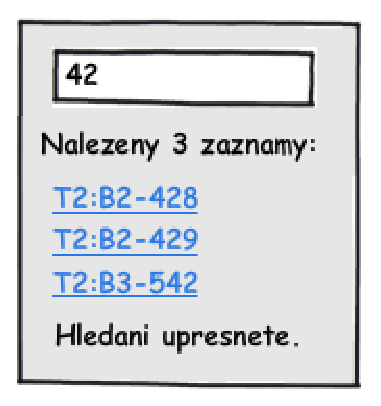
\includegraphics[width=30mm]{figures/LFviceVysledku}
% \caption{Nalezení několika výsledků}
% \label{fig:LFviceVysledku}
% \end{center}
% \end{figure}
% 
% \begin{figure}[ht]
% \begin{center}
% 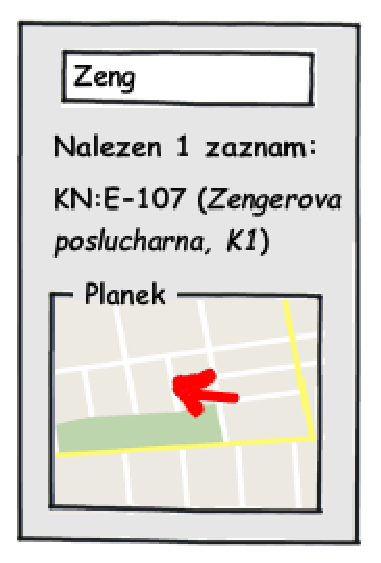
\includegraphics[width=30mm]{figures/LFjedinyVysledek}
% \caption{Nalezení jediného výsledku}
% \label{fig:LFjedinyVysledek}
% \end{center}
% \end{figure}
% 
% Aplikace by ještě měla poskytovat rozšířené vyhledávání s upřesněním hledaných míst a~zadáním výchozího bodu.
% 
% \noindent\textbf{Ostatní low fidelity prototypy jsou na přiloženém CD.}
% 
% 
% 
% \subsection{High fidelit prototyp}
% High fidelity prototypy jsou už sofistikovanějšími prototypy, jejich vytvoření tudíž trvá déle, ale přesto se je vyplatí udělat před finální aplikací -- nemají totiž plnou funkčnost konečné aplikace, nemusí ošetřovat vstupy a řešit nestandardní situace, takže se pořád vytvoří relativně rychle, přičemž už zadavateli dokáží realisticky demonstrovat finální práci s aplikací.
% 
% High fidelity prototyp jsem vytvořil pomocí XHTML, ECMAScriptu a CSS. Jedná se o~velmi vhodné technologie pro tvorbu prototypů -- rychle se vytvoří a snadno se pak upravují. Testování takto vytvořených prototypů je také příjemné -- v případě v prototypu nevyřešené situace lze snadno připravit výslednou situaci a testerovi ji na dálku bez nějakých komplikací podstrčit.
% 
% Na obrázku \ref{fig:HFviceVysledku} je vidět high fidelity prototyp ve stavu zobrazení více výsledků vyhledání.
% 
% \begin{figure}[ht]
% \begin{center}
% 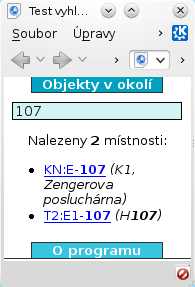
\includegraphics[width=30mm]{figures/HFviceVysledku}
% \caption{Nalezení několika výsledku}
% \label{fig:HFviceVysledku}
% \end{center}
% \end{figure}
% 
% Testování high fidelity prototypů je hlouběji popisované v kapitole o testování (viz \ref{sec:testhfp}).
% 
% \noindent\textbf{High fidelity prototyp je na přiloženém CD.}
% 
% 
% 
% \section{Případy užití}
% Případy užití (use cases) jsou scénáře popisující chování systému z pohledu vnějšího aktéra. Případy užití vymezují, kdo a co bude jak dělat a z tohoto základu se později sestaví funkční požadavky. Už ze zadání aplikace vyplývá potřeba jediného aktéra -- studenta. Základní případy užití jsou následující:
% \subsection{UC1: Hledání místnosti podle označení}
% \label{ssec:UChledaniMistnosti}
% \begin{description}
% \item[Aktéři:] Student.
% \item[Systém:] Navigační aplikace.
% \item[Vstupní podmínky:] ~\\*[-1.5em]
%  \begin{itemize}
%  \item Student je ve výchozí obrazovce aplikace.
%  \item Student se chce dostat do místnosti KN:E-9.
%  \end{itemize}
% \pagebreak
% \item[Hlavní scénář:] ~\\*[-1.5em]
%  \begin{enumerate}
%  \item Student vstoupí do vyhledávacího formuláře.
%  \item Student zadá písmeno \emph{K}.
%  \item Aplikace zobrazí seznam místností obsahujících písmeno \emph{K}.
%  \item Student zadá písmeno \emph{N}.
%  \item Aplikace zobrazí seznam místností obsahujících výraz \emph{KN}.
%  \item Student postupně zadá znaky \emph{:E-} a aplikace zúží seznam.
%  \item Student zadá číslici \emph{9}.
%  \item Aplikace zobrazí plán cílového patra s vyznačeným cílem.
%  \item Student dojde podle plánu k cíli.
%  \end{enumerate}
% \item[Poznámky:] ~\\*[-1.5em]
%  \begin{itemize}
%  \item Místnost by mělo jít stejným způsobem vyhledat i podle starého číslování a zažitých názvů.
%  \item Při zadání dvou a méně znaků lze kvůli nízkému výkonu zařízení a zachování přehlednosti zobrazovat upozornění na nutnost zadání více znaků.
%  \end{itemize}
% \end{description}
% 
% \subsection{UC2: Hledání neexistující místnosti}
% \begin{description}
% \item[Aktéři:] Student.
% \item[Systém:] Navigační aplikace.
% \item[Vstupní podmínky:] ~\\*[-1.5em]
%  \begin{itemize}
%  \item Student je ve výchozí obrazovce aplikace.
%  \item Student se chce dostat do místnosti KN:X-777.
%  \end{itemize}
% \item[Hlavní scénář:] ~\\*[-1.5em]
%  \begin{enumerate}
%  \item Student vstoupí do vyhledávacího formuláře.
%  \item Student postupně zadá znaky \emph{KN:X}.
%  \item Aplikace sdělí studentovi, že místnost neexistuje.
%  \end{enumerate}
% \item[Poznámky:] ~\\*[-1.5em]
%  \begin{itemize}
%  \item Podrobný popis postupu zadávání znaků a reakcí aplikace je v UC1 \ref{ssec:UChledaniMistnosti}.
%  \end{itemize}
% \end{description}
% 
% \pagebreak
% \subsection{UC3: Hledání kanceláře podle jména sídlícího vyučujícího}
% \begin{description}
% \item[Aktéři:] Student.
% \item[Systém:] Navigační aplikace.
% \item[Vstupní podmínky:] ~\\*[-1.5em]
%  \begin{itemize}
%  \item Student je ve výchozí obrazovce aplikace.
%  \item Student chce nalézt kancelář Zdeňka Míkovce.
%  \end{itemize}
% \item[Hlavní scénář:] ~\\*[-1.5em]
%  \begin{enumerate}
%  \item Student vstoupí do vyhledávacího formuláře.
%  \item Student zadá písmeno \emph{M}.
%  \item Aplikace zobrazí seznam místností obsahujících písmeno \emph{M}.
%  \item Student zadá písmeno \emph{í}.
%  \item Aplikace zobrazí seznam místností obsahujících výraz \emph{Mí}.
%  \item Student zadá písmeno \emph{k}.
%  \item Aplikace zobrazí plán cílového patra s vyznačeným cílem.
%  \item Student dojde podle plánu k cíli.
%  \end{enumerate}
% \end{description}
% 
% \subsection{UC4: Hledání nejbližšího nápojového automatu}
% \begin{description}
% \item[Aktéři:] Student.
% \item[Systém:] Navigační aplikace.
% \item[Vstupní podmínky:] ~\\*[-1.5em]
%  \begin{itemize}
%  \item Student je ve výchozí obrazovce aplikace.
%  \item Student se chce dostat k nejbližšímu nápojovému automatu.
%  \item Student se nachází před místností KN:E-9.
%  \end{itemize}
% \item[Hlavní scénář:] ~\\*[-1.5em]
%  \begin{enumerate}
%  \item Student vstoupí do vyhledávacího formuláře.
%  \item Student vyhledá místnost KN:E-9 podle UC1 \ref{ssec:UChledaniMistnosti}.
%  \item Aplikace zobrazí plán cílového patra s vyznačeným výchozím místem.
%  \item Student v plánu vyhledá požadovaný nápojový automat.
%  \item Student dojde podle plánu k cíli.
%  \end{enumerate}
% \end{description}
% 
% \subsection{UC5: Hledání za pomoci regulárních výrazů}
% \begin{description}
% \item[Aktéři:] Student.
% \item[Systém:] Navigační aplikace.
% \item[Vstupní podmínky:] ~\\*[-1.5em]
%  \begin{itemize}
%  \item Student je ve výchozí obrazovce aplikace.
%  \item Student se chce dostat do místnosti KN:E-9.
%  \end{itemize}
% \item[Hlavní scénář:] ~\\*[-1.5em]
%  \begin{enumerate}
%  \item Student vstoupí do vyhledávacího formuláře.
%  \item Student zadá znak \emph{-}.
%  \item Aplikace zobrazí seznam místností obsahujících znak \emph{-}.
%  \item Student zadá číslici \emph{9}.
%  \item Aplikace zobrazí seznam místností obsahujících výraz \emph{-9}.
%  \item Student zadá znak \emph{\$}.
%  \item Aplikace zobrazí seznam místností končících výrazem \emph{-9}.
%  \item Student si vybere ze seznamu místnost KN:E-9.
%  \item Aplikace zobrazí plán cílového patra s vyznačeným cílem.
%  \item Student dojde podle plánu k cíli.
%  \end{enumerate}
% \end{description}



\section{Funkční požadavky na serverovou aplikaci}
Funkčními požadavky (\textit{functional requirements}) jsou myšleny takové požadavky, které jsou zaměřeny na jednotlivé funkcionality. Pro serverovou aplikaci mezi ně patří především:
\begin{enumerate}
 \item Aplikace bude čerpat informace o názvech budov z předstíraného adaptéru.
 \item Aplikace bude čerpat informace o umístění budov z předstíraného adaptéru.
 \item Aplikace bude čerpat informace o názvech místností z předstíraného adaptéru.
 \item Aplikace bude čerpat informace o umístění místností z předstíraného adaptéru.
 \item Aplikace bude čerpat informace o rozvrzích místností z KOSapi (\url{http://kosapi.fit.cvut.cz/}). \todo{Vynechám -- chybí API.}
 \item Aplikace bude čerpat informace o rozvrzích studentů z formátu iCalendar.
 \item Aplikace bude čerpat informace o kontakech studentů z Usermap ČVUT (\url{http://usermap.cvut.cz/}).
 \item Aplikace bude čerpat informace o rozvrzích vyučujících z KOSapi (\url{http://kosapi.fit.cvut.cz/}). \todo{Vynechám -- chybí API.}
 \item Aplikace bude čerpat informace o kancelářích vyučujících z Usermap ČVUT (\url{http://usermap.cvut.cz/}).
 \item Aplikace bude čerpat informace o kontakech vyučujících z Usermap ČVUT (\url{http://usermap.cvut.cz/}).
 \item Aplikace bude čerpat informace o kancelářích neakademických pracovníků z Usermap ČVUT (\url{http://usermap.cvut.cz/}).
 \item Aplikace bude čerpat informace o kontaktech neakademických pracovníků z Usermap ČVUT (\url{http://usermap.cvut.cz/}).
 \item Aplikace bude čerpat informace o akcích \glsname{CVUT} z Kalendáře akcí ČVUT (\url{http://akce.cvut.cz/}).
 \item Aplikace bude čerpat informace o harmonogramu akademického roku z předstíraného adaptéru (na základě \url{http://fit.cvut.cz/}).
 \item Aplikace bude čerpat informace o datech \glsname{MAR} dostupných zdrojů (prozatím Orlík a Masarykova kolej, snaha o T9).
 \item Aplikace bude čerpat informace o jídelníčcích menz z Jídelníčků menz (\url{http://agata.suz.cvut.cz/jidelnicky/}).
 \item Aplikace bude čerpat informace o otvírací době menz z Jídelníčků menz (\url{http://agata.suz.cvut.cz/jidelnicky/}).
 \item Aplikace bude čerpat informace o otvírací době \glsname{NTK} z Národní technické knihovny (\url{http://www.techlib.cz/}).
 \item Aplikace bude čerpat informace o otvírací době Vydavatelství průkazů (\url{http://www.cvut.cz/informace-pro-studenty/prukazy}). \todo{Vynechám -- chybí API.}
 \item Aplikace bude čerpat informace o počtu lidí ve frontě ve Vydavatelství průkazů (\url{http://ke.customer.decent.cz/a021/mon/}).
 \item Vytvořte / nalezněte / sestavte z dílčích částí ontologii reprezentující výše uvedené informace.
 \item Informace získané z jednotlivých zdrojů převádějte dle výše požadované ontologie pro další zpracování do \glsname{RDF}.
 \item Aplikace uloží získané sémantické informace do databáze.
 \item Aplikace umožní vykonávat \glsname{SPARQL} dotazy nad uloženými daty.
\end{enumerate}

% \subsection{FR-S-1: Informace týkající se akcí ČVUT}
% Aplikace bude čerpat informace z webových stránek Kalendář akcí ČVUT (\url{http://akce.cvut.cz/}).
% \subsection{FR-S-2: Informace týkající se budov}
% Aplikace bude čerpat informace z předstíraného adaptéru obsahujícího informace týkající se budov.
% \subsection{FR-S-3: Informace týkající se místností}
% Aplikace bude čerpat informace z předstíraného adaptéru obsahujícího informace týkající se místností.
% \subsection{FR-S-4: Informace týkající se menz}
% Aplikace bude čerpat informace z webových stránek menz SUZ ČVUT (\url{http://agata.suz.cvut.cz/jidelnicky/}).
% \subsection{FR-S-5: Informace týkající se osob spjatých s ČVUT}
% Aplikace bude čerpat informace z webových stránek Usermap ČVUT (\url{http://usermap.cvut.cz/}).
% \subsection{FR-S-6: Převod informací do \emph{RDF}}
% Informace získané z jednotlivých zdrojů převádějte pro další zpracování do \emph{RDF}.
% \subsection{FR-S-7: Perzistentní uložení do databáze}
% Aplikace uloží získané informace do databáze.
% \subsection{FR-S-8: \emph{SPARQL} endpoint}
% Aplikace umožní vykonávat \emph{SPARQL} dotazy nad uloženými daty.


\section{Nefunkční požadavky na serverovou aplikaci}
Nefunkčními požadavky (\textit{non-functional requirements}) jsou myšleny takové požadavky, které jsou zaměřeny na dílo jako celek, nikoliv na jednotlivé funkcionality. Pro serverovou aplikaci mezi ně patří především:

\begin{enumerate}
 \item Aplikaci naprogramujte v \emph{JavaScript}u.
 \item Pro běh serveru využijte \emph{Node.js}.
 \item Sémantická data ukládejte do takového úložiště, aby nad ním bylo možné vykonávat dotazy přímo (případně přes nezávislého prostředníka) a nebylo nutné přistupovat přes vlastní aplikaci.
 \item Práce nemusí nutně obsáhnout celou zpracovávanou doménu, je ale žádané, aby kvalitně zpracovala hlavní scénáře využití a nebránila dalšímu rozšiřování.
 \item Zveřejněte aplikaci a její data pod svobodnými licencemi z rodin \emph{\glsname{GNU}}, \emph{Creative Commons} a kompatibilními, aby byl umožněn další rozvoj nezávislý na původním autorovi.
\end{enumerate}

% \subsection{NFR-S-1: Aplikaci naprogramujte v \emph{JavaScript}u}
% V poslední době dochází k prudkému rozvoji \emph{JavaScript}u a dá se mu do budoucna předpovídat vyšší nasazení, aplikaci tedy naprogramujte v \emph{JavaScript}u.
% \subsection{NFR-S-2: Pro běh serveru využijte \emph{Node.js}}
% Pro běh aplikace využijte systém \emph{Node.js} a naučte se práci s touto novou a progresivní technologií.
% \subsection{NFR-S-3: Využijte úložiště sémantických dat}
% Sémantická data ukládejte do takového úložiště, aby nad ním bylo možné vykonávat dotazy přímo (případně přes nezávislého prostředníka) a nebylo nutné přistupovat přes vlastní aplikaci.
% \subsection{NFR-S-4: Dejte přednost kvalitě zpracování}
% Práce nemusí nutně obsáhnout celou zpracovávanou doménu, je ale žádané, aby kvalitně zpracovala hlavní scénáře využití a nebránila dalšímu rozšiřování.
% \subsection{NFR-S-5: Svobodné licence}
% Zveřejněte aplikaci a její data pod svobodnými licencemi z rodin \emph{GNU}, \emph{Creative Commons} a kompatibilními, aby byl umožněn další rozvoj nezávislý na původním autorovi.



\section{Funkční požadavky na mobilní aplikaci}
Funkčními požadavky (\textit{functional requirements}) jsou myšleny takové požadavky, které jsou zaměřeny na jednotlivé funkcionality. Pro mobilní aplikaci mezi ně patří především:

\begin{enumerate}
 \item Aplikace umožní pokročilému uživateli zadat vlastní \glsname{SPARQL} dotaz. Ten se odešle na server, kde se zpracuje, a výslek se navrátí uživateli.
 \item Pro méně znalé uživatele \glsname{SPARQL} a pro uživatele minimalizující použití klávesnice vytvořte předpřipravené dotazy pro základní scénáře použití aplikace.
 \item Implementujte funkcionalitu umožňující určení aktuální pozice a její předání dalšímu zpracování.
 \item Aplikace dokáže na mapě vizualizovat určitou pozici.
%  \item Aplikace umožní vizualizovat polohu uživatele na základě GPS souřadnic.
%  \item Aplikace umožní vizualizovat polohu uživatele na základě známého blízkého objektu (např. čísla místnosti).
%  \item Aplikace umožní vizualizovat polohu hledaného objektu.
 \item Aplikace dokáže vizualizovat \glsname{HTML} data nebo data jako \glsname{HTML}.
 \item Aplikace bude poskytovat nápovědu pro snazší použití.
 \item Aplikace bude postavená nad daty reprezentovanými výše uvedenou ontologií.
\end{enumerate}

% \subsection{FR-M-1: Možnost vlastních \emph{SPARQL} dotazů}
% Aplikace umožní pokročilému uživateli zadat vlastní \emph{SPARQL} dotaz. Ten se odešle na server, kde se zpracuje, a výslek se navrátí uživateli.
% \subsection{FR-M-2: Výběr předpřipravených dotazů}
% Pro méně znalé uživatele \emph{SPARQL} a pro uživatele minimalizující použití klávesnice vytvořte předpřipravené dotazy pro základní scénáře použití aplikace.
% % \subsection{FR-M-: Vyhledání místností}
% % Připravte aplikaci mimo předem nespecifických dotazů i na ty požadující vyhledání místností. 
% % \subsection{FR-M-: Vyhledání bodů zájmu}
% % Připravte aplikaci mimo předem nespecifických dotazů i na ty požadující vyhledání bodů zájmu. 
% \subsection{FR-M-3: Určení aktuální pozice}
% Implementujte funkcionalitu umožňující určení aktuální pozice a její předání dalšímu zpracování.
% \subsection{FR-M-4: Vizualizace pozice}
% Aplikace dokáže na mapě vizualizovat určitou pozici.
% \subsection{FR-M-5: Vizualizace \emph{HTML} dat}
% Aplikace dokáže vizualizovat \emph{HTML} data nebo data jako \emph{HTML}.
% \subsection{FR-M-6: Nápověda}
% Aplikace bude poskytovat nápovědu pro snazší použití.


\section{Nefunkční požadavky na mobilní aplikaci}
Nefunkčními požadavky (\textit{non-functional requirements}) jsou myšleny takové požadavky, které jsou zaměřeny na dílo jako celek, nikoliv na jednotlivé funkcionality. Pro mobilní aplikaci mezi ně patří především:

\begin{enumerate}
 \item Aplikaci vytvořte v \glsname{HTML}5, aby byla na současných, obzvláště mobilních, zařízeních multiplatformní.
 \item Aplikace bude funkční v prohlížečích na nejnovějších verzích \glsname{OS} Android, iOS a Symbian.
 \item Aplikace bude funkční v majoritních desktopových prohlížečích.
 \item Při vývoji se zaměřte i na použitelnost, aplikaci by měl být schopný, po krátkém zaškolení, používat jakýkoliv běžný student Fakulty informačních technologií.
 \item Snažte se nabízet alternativy k zadávání dlouhých textů, aby byla usnadněna obsluha uživatelům mobilních zařízení bez hardwarových klávesnic.
 \item Práce nemusí nutně obsáhnout celou zpracovávanou doménu, je ale žádané, aby kvalitně zpracovala hlavní scénáře využití a nebránila dalšímu rozšiřování.
 \item Zveřejněte aplikaci a její data pod svobodnými licencemi z rodin \glsname{GNU}, \emph{Creative Commons} a kompatibilními, aby byl umožněn další rozvoj nezávislý na původním autorovi.
 \item Aplikace umožní využití off-line. \todo{Vynechám -- muselo by se složitě indexovat.}
\end{enumerate}


% \subsection{NFR-M-1: Multiplatformnost}
% Aplikaci vytvořte v \emph{HTML5}, aby byla na současných, obzvláště mobilních, zařízeních co nejvíce multiplatformní. Bude funkční minimálně v nejnovějších verzích OS Android, iOS a Symbian.
% \subsection{NFR-M-2: Použitelnost}
% Při vývoji se zaměřte i na použitelnost, aplikaci by měl být schopný, po krátkém zaškolení, používat jakýkoliv běžný student Fakulty informačních technologií.
% \subsection{NFR-M-3: Omezené použití klávesnice}
% Snažte se nabízet alternativy k zadávání dlouhých textů, aby byla usnadněna obsluha uživatelům mobilních zařízení bez hardwarových klávesnic.
% % \subsection{NFR-M-: Offline provoz}
% \subsection{NFR-M-4: Dejte přednost kvalitě zpracování}
% Práce nemusí nutně obsáhnout celou zpracovávanou doménu, je ale žádané, aby kvalitně zpracovala hlavní scénáře využití a nebránila dalšímu rozšiřování.
% \subsection{NFR-M-5: Svobodné licence}
% Zveřejněte aplikaci a její data pod svobodnými licencemi z rodin \emph{GNU}, \emph{Creative Commons} a kompatibilními, aby byl umožněn další rozvoj nezávislý na původním autorovi.




% \section{Návrh řešení}
% Návrh (design) této aplikace neprobíhal příliš dlouho, aplikace nemá být nijak složitá a~rozsáhlá, ani není po stránce návrhu nějak výjimečná, takže se zde návrhu příliš věnovat nebudeme.
% 
% \subsection{Vyhledávání}
% Stěžejní funkcí má být vyhledávání, to je zároveň i stěžejním bodem návrhu. Je nutné splnit všechny funkční i nefunkční požadavky, kde je vyhledávání silně zastoupeno.
% 
% Vyhledávací algoritmus by měl fungovat následovně, začnu popisovat od databáze, ze které se vyhledává. Databáze bude obsahovat mnoho (až tisíce) záznamů a je proto v mobilním prostředí nutné, aby bylo vyhledávání, včetně samotné databáze, optimalizované. Aby došlo v průběhu vyhledávání ke snížení toku dat algoritmem, provedeme dekompozici databáze a vyčleníme hledatelné položky (označení učeben, jména vyučujících...) stranou, můžeme je ještě abecedně seřadit. Tady optimalizace databáze prozatím končí a můžeme se přesunout k samotnému algoritmu.
% 
% Původně jsem zamýšlel vyhledávat binárním půlením nebo jiným algoritmem optimalizovaným pro seřazený seznam, přišel ale požadavek na vyhledávání pomocí regulárních výrazů a tím tato možnost odpadla -- je potřeba projít všechny místnosti a zkontrolovat každou položku.
% 
% Regulární výrazy se nám většinou postarají i o nerozlišování velikosti písmen, takže si jimi alespoň pomůžeme k dalšímu požadavku.
% 
% Při kontrole položky můžeme zároveň vyřešit i požadavek na hledání bez diakritiky, zase ale musíme optimalizovat. Nebylo by složité vytvořit algoritmus, který zkouší nahradit každé písmeno bez diakritiky jeho diakritickými variantami, tím by nám ale výrazně narostla náročnost algoritmu, slovo \emph{mistnost} by tak najednou odpovídalo sto dvaceti osmi výrazům (\emph{mistnost}, \emph{m\textbf{í}stnost}, \emph{mi\textbf{š}tnost}, \emph{m\textbf{íš}tnost}...), tolikrát ale nezvládneme se současným výkonem mobilních zařízení celou databázi prohledat.\footnote{V praxi není toto omezení tolik markantní, označení místností obsahuje spíše znaky bez diakritiky. Vyhledávané osoby ale diakritiku ve jménech mají, takže toto omezení zachováme.} Umožníme vyhledávat buď jen s diakritikou, nebo bez, čímž slovo \emph{mistnost} bude odpovídat pouze dvěma výrazům (\emph{mistnost} a \emph{m\textbf{í}stnost}). Vyřešíme to následovně, všechny diakritiku obsahující položky v již dříve zmíněném duplicitním seznamu uložíme do tohoto seznamu ještě jednou, tentokrát bez diakritiky.
% 
% Nalezeným položkám přiřadíme místnosti, které reprezentují (například položce \emph{Josef Vomáčka} místnost \emph{KN:E-108}), vyřadíme duplicitní místnosti a seřadíme je podle abecedy.
% 
% \subsection{Navigace}
% Zpočátku jsme v analýze uvažovali o vyznačení cesty z výchozího bodu do cílového, to by ale, mimo náročného algoritmu, dost uživateli v některých věcech přitížilo. V první řadě by přišel o mnoho místa malého displeje formulářem pro zadání výchozího bodu, v druhé řadě by bylo vytvoření optimálního algoritmu hledajícího cestu pravděpodobně nemožné (viz \ref{subs:UNcestaAplikaci}) a špatná cesta by se uživateli nemusela líbit. Problém v tom naštěstí pravděpodobně nebude, budovy nejsou stavěné jako bludiště a navigace po nich s plánkem není problém.
% 
% Vyhledáním místnosti získá aplikace cíl, ke kterému je potřeba uživatele navést. Dobrým řešením je ukázat uživateli plán cílového patra s vyznačeným cílem, orientačními body, schodišti (a výtahy) a vstupy do budovy (s~rozdíly pater). Uživatel se tak dokáže v plánu zorientovat, i kdyby se mu to doposud nepodařilo, schodiště (většinou vedou budovou každým patrem) a vchody do budovy (většinou jsou maximálně dva) k tomu velmi pomohou. Plán pouze cílového patra proto, že cestu po schodech nemá cenu vizualizovat (dokonce je to spíše nevhodné) a v rámci výchozího patra je většinou zcela zřejmé, jak se ke schodům dostat. Uživatel se tedy zvládne dostat do uvedeného patra a tam už podle plánu k hledané místnosti sám bez větších komplikací.


% (f) Popis implementace/realizace produktu se zaměřením na nestandardní části řešení.

\chapter{Realizace}
% Popis implementace/realizace se zaměřením na nestandardní části řešení.
Během implementace (\textit{implementation}) se objevila celá řada zádrhelů, z nichž mnoho souviselo s doposud ne zcela zdokumentovanými a odladěnými technologiemi, přesto pro mne byla realizace velmi přínosná -- neustálým hledáním různých řešení a alternativ jsem nutně narazil na mnoho dalších zajímavých postřehů a nápadů. Kapitola se zabývá řešenými problémy, komplikacemi a celá je protkána implementací bezpečnosti. % , potenciální aplikací v ideálním světě

\section{Serverová aplikace}
Když se zpětně ohlížím za implementací serverové aplikace, náročná objektivně vůbec nebyla, osobně jsem ale žádnou z používaných technologií / knihoven\dots v té době neznal, takže mi náročnost přišla enormně vysoká. Rozsah popisu realizace serverové aplikace je tak krátký -- mnoho objektivně zajímavých míst se v ní nevyskytlo.

Realizováno bylo pouze zpracování čtyř rozličných typů zdrojů -- implementace ostatních by byla dlouhotrvajícím opakováním stejných postupů a práci by moc neobohatila.

\subsection{Řešené problémy}
V době, kdy byl vytvořený návrh, bylo vytvoření aplikace už poměrně snadné. Popíšu tedy jen ve stručnosti několik základních částí řešení.

\subsubsection{Zpracování zdroje}
Proces zpracování zdroje je poměrně přímočarý. Nejprve je zdroj po jednotlivých \textit{chuncích} stažen, následně sestaven:
\begin{verbatim}
var http = require('http'); //načtení modulu

var request = http.get({
    host: 'akce.cvut.cz',
    path: '/index.php'
});
request.on('response', function (r) {
    var data = '';
    r.on('data', function (chunk) {
        data += chunk;
    });
    r.on('end', function () {
        //zpracování dat
    });
});
\end{verbatim}
Poté je pro snadnou a spolehlivou manipulaci vytvořen model dokumentu daného formátu, se kterým se pak pracuje, například pro \glsname{HTML} nebo \glsname{XML}:
\begin{verbatim}
var $ = require('jquery');
var jqo = $(data);
jqo.find('#content span.location').text();
\end{verbatim}
Pro iCalendar:
\begin{verbatim}
var icalendar = require('icalendar');
var ical = icalendar.parse_calendar(data);
ical.events()[0].properties.LOCATION;
\end{verbatim}
Získaná data jsou pak ukládána do grafového úložiště:
\begin{verbatim}
var rdfstore = require('rdfstore');

var store = rdfstore.create(config, function (store) {
    var graph = store.rdf.createGraph();

    store.rdf.setPrefix(
        "lode", "http://linkedevents.org/ontology/");

    for (var e in ical.events()) {
        var event = store.rdf.createNamedNode(
            ical.events()[e].properties.URL.value);

        graph.add(
            store.rdf.createTriple(
                event,
                store.rdf.createNamedNode(
                    store.rdf.resolve("rdf:type")),
                store.rdf.createNamedNode(
                    store.rdf.resolve("lode:Event"))
            )
        );

        //další informace zpracovávány obdobně
    }

    store.insert(graph, function () {
        console.log("Graph has been inserted.")
    });
});
\end{verbatim}
Zdrojový kód je v tomto případě dobře čitelný, žádné další komentáře tedy asi nepotřebuje. Za povšimnutí pouze stojí asynchronní charakter celé aplikace -- nikde se neblokují zdroje zbytečně a nemůže se stát, že by nějaká událost předběhla jinou.

\subsubsection{Zdroje uživatelských jmen}
Nepodařilo se mi nalézt vhodný zdroj uživatelských jmen vyučujících a neakademických pracovníků. Zatímco uživatelská jména studentů jsou zveřejněna na \url{https://timetable.fit.cvut.cz/public/cz/studenti/}, na obdobné stránce věnované učitelům, \url{https://timetable.fit.cvut.cz/public/cz/ucitele/}, jsou pouze tituly, křestní jména a příjmení -- tedy nic, co by bylo vhodným identifikátorem. Zdroj uživatelských jmen neakademických pracovníků se mi nepodařilo nalézt žádný. Vzhledem k plánovanému budoucímu napojení aplikace na KOSapi (\url{http://kosapi.fit.cvut.cz/}), až získá přístup do \glsname{KOS}, byly jako dočasné řešení zvoleny soubory obsahující jména a uživatelská jména všech osob.

\subsubsection{Routování}
Aplikace je serverem\footnote{Pozor, zde je důležité vzít v potaz vymezení pojmů z poznámky \ref{fnt:aplikace} na straně \pageref{fnt:aplikace} -- aplikace, o které je řeč, je \textit{serverovou aplikací} v užším slova smyslu -- není nazývána \textit{serverovou aplikací} proto, že by nutně musela být serverem, ale proto, že je jednou z komponent serverového řešení. Že je tedy také serverem je pouze shoda náhod.} a obsluhuje se \glsname{HTTP} požadavky, je tak dosaženo větší univerzálnosti. Například pro aktualizaci osob spjatých s fakultou je třeba odeslat požadavek \texttt{GET} na \glsname{URL} \texttt{http://\linebreak[0]localhost:1337/\linebreak[0]osoby/}, na které je server spuštěný. Zpracování takového požadavku je vyřízeno následujícím kódem ze \textit{spouštěcího} souboru aplikace:
\begin{verbatim}
var express = require('express'); //načtení frameworku express

var app = express.createServer(); //vytvoření serveru

app.get('/osoby/:login?', function (req, res) {
    require('./sources/usermap.js').process(req.params.login);
    res.send("OK: Source enqueued for processing.");
});

//další zdroje zpracovávány obdobně

app.get('*', function (req, res) { //neodchycené cesty
    res.send("Error: Service not found.", 404);
});

app.listen(1337); //spuštění aplikace na portu 1337
\end{verbatim}
V těchto několika řádcích je vytvořený celý server zpracovávající příchozí požadavky. Na pátém řádku je řečeno, že cesta směřující do \textit{segmentu} osoby bude touto metodou odchycena. Odchycen bude i další, nepovinný, segment, který bude uložený do proměnné \texttt{login}. Je tedy možné volat i \glsname{URL} \texttt{http://\linebreak[0]localhost:1337/\linebreak[0]osoby/\linebreak[0]molnaja2/}, aniž by došlo k odchycení dvanáctým řádkem, který klientovi vrátí patřičnou chybu.

Uvnitř metody je na prvním řádku vyžadováno zavolání metody \texttt{process()} z uvedeného souboru s parametrem \texttt{login}. V této metodě je na základě přítomnosti parametru rozhodnuto, jestli se mají zpracovat všechny osoby nebo jen jedna konkrétní. Na druhém řádku je klientovi odesláno oznámení o úspěšném přijetí požadavku.

\subsubsection{Nastavení plánovače}
\label{sec:server:scheduler}
Vzhledem k výše uvedené obsluze \textit{serverové aplikace} \glsname{HTTP} požadavky je možné plánovač reprezentovaný cronem jednoduše nastavit, například:
\begin{verbatim}
# aktualizace jidelnicku kazdy den 3 minuty po zverejneni
3 9,10,16,17 * * * user curl localhost:1337/jidelnicky/\
               2>&1 1> jidelnicky.all.log 2> jidelnicky.err.log

# aktualizace osob kazdy den 10 minut po druhe hodine
10 2 * * * user curl localhost:1337/osoby/\
               2>&1 1> osoby.all.log 2> osoby.err.log

# aktualizace akci 10 minut po kazde sude hodine
10 */2 * * * user curl localhost:1337/akce/\
               2>&1 1> akce.all.log 2> akce.err.log

# aktualizace rozvrhu kazdy den 10 minut po druhe hodine
10 2 * * * user curl localhost:1337/rozvrh/\
               2>&1 1> rozvrh.all.log 2> rozvrh.err.log
# aktualizace rozvrhu v dobe tvorby 10 minut po kazde hodine
10 * * 6,9,10,1,2 * user curl localhost:1337/rozvrh/\
               2>&1 1> rozvrh.all.log 2> rozvrh.err.log
\end{verbatim}
Prvních pět parametrů udává čas vykonání akce (minuta, hodina, den měsíce, měsíc, den týdne), šestý uživatele, zbytek je vykonání příkazu -- odeslání požadavku a \textit{zalogování} výsledku.

% \subsection{Implementace bezpečnosti}

\subsection{Komplikace}
Během implementace serverové aplikace vyvstalo několik komplikací, které bylo třeba vyřešit:

\subsubsection{Převod kódování}
Node.js vznikl až po prosazení \glsname{UTF}-8, dá se tedy předpokládat, že bude toto kódování podporovat. Předpoklad je to samozřejmě, i dle dokumentace \cite{NodeEncoding}, správný; horší je to ale, dle stejného zdroje, s ostatními kódováními. Samotný Node.js může data v nich převádět do \textit{bufferu}, který pak lze následně, například pomocí systémového programu iconv volaného prostřednictvím knihovny node-iconv, převést do správného kódování.

Problém vyvstává u vysokoúrovňových nástrojů, které například dokáží jednoduše stáhnout cizí internetovou stránku a předpřipravit ji k následnému zpracování -- pokud je u těchto nástrojů vrácen třeba \glsname{DOM}, v případě, že pocházela stránka ze zdroje, který využíval s Node.js nekompatibilní kódování, řekněme Windows-1250, převod kódování už nelze zpětně ovlivnit. Při zpracovávání některých stránek jsem tak musel zůstat u nízkoúrovňových nástrojů.

\subsubsection{Špatně formované XML}
Při práci se sémantickým úložištěm rdfstore-js jsem narazil na špatně formované \glsname{XML}. Chybu jsem identifikoval -- jednalo se o sekvenci \verb|<literal>>| v některých případech generovaného \glsname{XML}, nalezl chybu v kódu, nahlásil a odeslal \textit{patch}. V současné době je chyba již odstraněna \cite{IssueLiteral}.

% \subsection{Ideální implementace}


\section{Mobilní aplikace}
Pod pojmem \textit{mobilní aplikace} se skrývá aplikace pevně nezávislá na výše uvedené \textit{serverové}. Jejím hlavním cílem je sloužit studentovi \glsname{FIT} \glsname{CVUT} jako průvodce, zároveň má ale plnit i účel ukázky využití \glsname{SPARQL} endpointu vytvořeného v \textit{serverové} části.

\subsection{Řešené problémy}
Implementace mobilní aplikace přinesla mnoho menších problémů, které bylo třeba vyřešit. Mezi nejzajímavější patří:

\subsubsection{Vyhledávání v navigaci}
Aby bylo vyhledávání pro uživatele co nejvíce přívětivé, je třeba mu věnovat hodně pozornosti. Změnou vyhledávací fráze (stiskem klávesy, stiskem vyhledávacího tlačítka, odesláním formuláře, změnou formuláře) je vyvoláno hledání, kde jsou nejprve z vyhledávané fráze ořezány (počáteční a koncové) bílé znaky a následně je převedena do dvou regulárních výrazů -- první je tvořený frází tak, jak je zadána, druhý je normalizovaný. Normalizací je odstraněna diakritika, interpunkce a zbylé bílé znaky. Nyní už jsou prohledána všechna místa z databáze, nejprve na přítomnost prvního zmiňovaného regulárního výrazu, poté se normalizují a testují na druhý regulární výraz. Ve vyhledávání nezáleží na velikosti písmen.

V průběhu celého procesu jsou zpracovávány krajní situace a řešena otázka uživatelské přívětivosti -- v případě chyby v regulárním výrazu je uživateli nabídnuta oprava, jsou vypisována hlášení o průběhu vyhledávání a dle počtu nalezených výsledků jsou tyto prezentovány -- jediný výsledek je rovnou zobrazen, více výsledků se vypíše a uživatel má možnost si dále z nich vybrat, případně pokračovat v zadávání hledané fráze.

\subsubsection{Mapa v navigaci}
Mapa v navigaci je tvořena \glsname{SVG} obrázkem, se kterým je manipulováno JavaScriptem. Z mapy je zobrazována pouze výseč, která je navíc dle potřeby škálována -- to nutně vede k mnoha různým algoritmům:
\begin{itemize}
 \item Změna velikosti mapy v případě změny velikosti okna (minimalizací prohlížeče nebo třeba překlopením mobilního zařízení) -- velikost mapy se totiž automaticky nastavuje na velikost obrazovky, aby nebyla zbytečně velká a přesto ji mohl mít uživatel zobrazenou na celém displeji.
 \item Posun zobrazované výseče po vyžádání uživatelem nebo na nalezený objekt. Je nutné brát v potaz aktuální škálování mapy.
 \item Škálování mapy vyžádané uživatelem nebo dle nalezeného objektu. Je nutné brát v potaz aktuální zobrazovanou výseč.
 \item Zjištění pozice vykonaného gesta -- je odvozována na základě pozice obalového elementu, zjišťování pozice z mapy dávalo vlivem různých implementací jiné výsledky napříč prohlížeči.
 \item Převedení zeměpisných souřadnic na místo na mapě -- je realizováno prostým odvozením od souřadnic rohů mapy, zakřivení země je zanedbáno, pro dané účely tento přístup dostačuje.
\end{itemize}
V mapových podkladech jsou z důvodu velkého rozsahu dopodrobna na úrovni místností rozpracovány pouze první a třetí podlaží budovy T9 a na úrovni budov pouze dejvický kampus.

% \subsubsection{Optimalizace}
% vyhledávání

\subsubsection{Rozdílné DOM u HTML a SVG}
\glsname{SVG} je, co se týče návrhu \glsname{DOM}, komplikovanější, než \glsname{HTML} -- zatímco u \glsname{HTML} stačí k hodnotě atributu v \glsname{DOM} přímo přistoupit, v \glsname{SVG} se musí zpravidla ještě o dvě úrovně níže, tedy třeba místo k \texttt{.width} se musí přistupovat k \texttt{.width.baseVal.value}. Při implementaci to bylo třeba brát v potaz.

\subsubsection{Malá velikost displeje}
Ačkoliv je toto omezení u mobilních zařízení zřejmé, nic to nemění na faktu, že se s ním musí neustále počítat a je třeba vybírat vhodné komponenty a ty vhodně rozvrhovat. Malá velikost displeje byla omezením i z opačného hlediska -- prsty jsou u dotykových telefonů, vzhledem k velikosti displeje, poměrně velké a ovládací prvky tak musí být dostatečně rozměrné, což konzumuje další místo. Mým cílem proto bylo vizualizovat jen to nejnutnější.

\subsubsection{Různé typy polohovacích zařízení}
Různá zařízení poskytují různé ovládací prvky využívající různé principy, aplikaci je ale potřeba přizpůsobit pro všechny najednou. Jiné je ovládání pro myš (touchpad, trackpad\dots), jiné pro klávesy a jiné pro dotyková zařízení -- právě s těmi je problém -- v rámci použitých technologií ještě nebyl vytvořen žádný standard pro zpracování zpracování gest, proto bylo nutné umístit nad mapu výrazné ovládací prvky.

\subsubsection{Dynamické načítání lokálních souborů}
Z bezpečnostních důvodů došlo v minulosti v prohlížečích k zamezení načítání jakýchkoliv souborů, mimo JavaScriptu, z jiných zdrojů, než ze kterých stránka pochází. To v některých případech\footnote{Příkladem je Google Chrome a jeho základ Chromium \cite{BugChromeOrigin}.} přerostlo v zamezení dynamického načítání jakýchkoliv lokálních souborů -- jejich zdroj nemá žádnou hodnotu (\texttt{null}), takže je nelze načíst. Aby byla zachována možnost offline využití aplikace na větší skupině zařízení, byla aplikace přepsána na jediné možné řešení -- explicitní uvedení všech potenciálně vkládaných souborů, což značně omezilo modularitu aplikace.

Například v případě \glsname{SVG} je široká nabídka volby -- lze vložit JavaScriptem do elementů \texttt{img} (\texttt{<img src="map.svg"\ />}), \texttt{embed} (\texttt{<embed src="map.svg"\ />}), \texttt{object} (\texttt{<object type="image/svg+xml"\ data="map.svg"\ />}), \texttt{iframe} (\texttt{<iframe src="map.svg"\ />}), pokud je pak umožněna manipulace s obsahem pomocí JavaScriptu, tak jen velice neohrabaně. Další možností je vložit \glsname{SVG} přímo do \glsname{HTML} kódu -- v případě dynamicky generovaného kódu by bylo vhodné celý soubor načíst a na místo vložit, jenže zde narážíme na problém z předchozího odstavce -- některé prohlížeče to neumožní. Zbývá tedy poslední řešení -- celý soubor převést do JavaScriptového řetězce, uložit do proměnné a vložit z ní. Jedině tak zle vložit do stránky \glsname{SVG} soubor, aby s ním pak bylo snadné manipulovat prostřednictvím jediného \glsname{DOM}.

% \subsubsection{Otevírání lokálních souborů}
% Omezení zmíněná v předchozím odstavci stupňuje až do extrémů mobilní prohlížeč Chrome Beta, který nepovolí ani přímé otevření lokálního souboru. \todo{Ověřit, možná nefunguje celé Chrome\dots}

\subsubsection{Zpracování Cross-Origin zdrojů}
\label{sec:mobil:cross-origin}
Aplikace potřebuje získávat a zpracovávat cizí zdroje -- aby poskytovala aktuální informace, nevystačí si jen s lokálním úložištěm, musí přímo k jejich původci. To je ale zpravidla v doméně použitých technologií komplikované -- webové prohlížeče z bezpečnostních důvodů nepovolují k cizím zdrojům přístup (výjimkou je například JavaScript -- více dále), takže je třeba danou situaci řešit.

\glsname{SPARQL} endpoint ze serverové aplikace, tedy hlavní předpokládaný zdroj informací, máme plně ve své režii, takže na něm můžeme povolit \gls{CORS}, tedy technologii umožňující serveru zpřístupnit své zdroje i z jiné domény. Jediný problém je u špatné podpory některých prohlížečů.

Z již dříve popsaných důvodů, tedy malého rozsahu sémantické databáze, ale finální aplikace podporuje mimo přístupu k samotnému \glsname{SPARQL} endpointu i přímý přístup k původním zdrojům. Zde vyvstává problém -- na cizích zdrojích \glsname{CORS} povolit nemůžeme, je tedy třeba najít jiné řešení. Tím je \gls{JSONP}, tedy postup umožňující získat přes JavaScriptový soubor (ten má výjimku) data ve formátu \glsname{JSON} obalená funkcí námi zvoleného jména, která je po stažení zdroje v prohlížeči vykonána, a tím jsou aplikaci předána data ke zpracování.

\glsname{JSONP} sám o sobě ale nic nevyřeší -- je k němu stejně tak potřeba mít uzpůsobený server. Tady nám pomůže jednoduchá \textit{proxy}, které zadáme požadavek na zdroj, ona ho získá a odešle nazpátek. I zde by nakonec nemuselo být \glsname{JSONP}   potřeba, proxy zase bude v naší režii (v případě existence jiné vhodné, v cizí), a šlo by pak použít \glsname{CORS}; protože se ale jedná o dočasné řešení v době, kdy ještě některé menšinové prohlížeče \glsname{CORS} nepodporují, rozhodl jsem se si vyzkoušet implementaci další technologie.

Z veřejně k použití dostupných proxy lze využít například server Yahoo! využívaný pro \textit{Yahoo! Query Language} (\url{http://developer.yahoo.com/yql/}) -- na něm je založeno jQuery rozšíření cross-domain-ajax (\url{https://github.com/padolsey/jQuery-Plugins/}), dále je možné na vlastním serveru použít nějaké hotové řešení, například \textit{AJAX Cross Domain} (\url{http://www.ajax-cross-domain.com/}), nebo si vše od základu vytvořit sám.

Rozhodl jsem se pro třetí možnost -- veřejně dostupná řešení nenabízejí potřebné možnosti konfigurace, mezi již hotovými řešeními se mi nepodařilo nalézt vhodné pro konkrétní použití, takže jsem si vytvořil proxy vlastní.\footnote{Byla tedy přidána další serverová aplikace do již tak terminologicky složité situace. Z tohoto důvodu se u zmíněného serveru držím označení \textit{proxy}.}

Proxy je požádána o zprostředkování zdroje, na základě \textit{whitelistu} je rozhodnuto o jeho poskytnutí -- z bezpečnostních důvodů je zamezen přístup ke všem mimo nutně potřebných serverů. Zdroj proxy stáhne, převede na přednastavené kódování (v rámci JavaScriptu nejsou převody snadné, dojde tak k výraznému usnadnění mobilní aplikaci) a před odesláním odpovědi je zdroj pročištěn -- za využití knihovny \textit{HTML Purifier} je zdroj zvalidněn a je z něj odstraněno vše, co není explicitně dalším \textit{whitelistem} povoleno -- skripty, obrázky, rámce, další zdroje, potenciálně škodlivé atributy a elementy\dots V případě chyby je uživateli (mobilní aplikaci) navráceno příslušné chybové hlášení.

\subsubsection{Uživatelské rozhraní}
Tvorba uživatelského rozhraní mobilní aplikace nepřinesla, mimo tvorby mapy a zpracování cizích zdrojů, žádné zvlášť komplikované úkony. Tvorba mapy byla již popsána. Zpracování cizích zdrojů bylo vyžadováno pro jejich různorodost -- každý poskytoval informace v jiném formátu, transformoval jsem je tedy do obdobnějších reprezentací vhodných pro mobilní zařízení. Pro ilustraci přikládám obrázek \ref{fig:mobil:android:pruvodce} znázorňující uživatelské rozhraní mobilního průvodce.
\begin{figure}[h]
 \centering
 \setlength\fboxsep{0pt}
 \setlength\fboxrule{0.5pt}
 \fbox{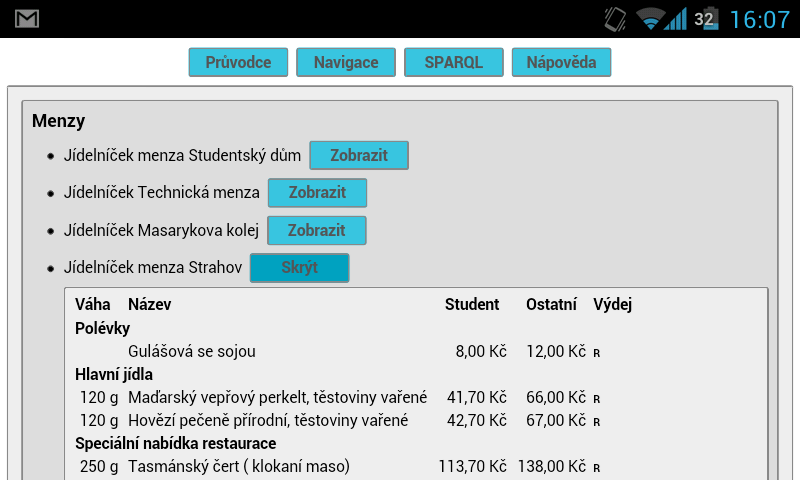
\includegraphics[width=9.1cm]{./figures/android-pruvodce.png}}
 % android-pruvodce.png: 800x480 pixel, 72dpi, 28.22x16.93 cm, bb=0 0 800 480
 \caption{Snímek obrazovky aplikace v prohlížeči platformy Android}
 \label{fig:mobil:android:pruvodce}
\end{figure}



\subsection{Komplikace}
Během implementace mobilní aplikace se objevily i komplikace, mimo očekávaných, již zmíněných v předchozí části, mezi ně patřilo:

\subsubsection{Chyby prohlížečů v implementaci specifikací}
Při práci jsem několikrát narazil na situaci, kdy určitá vlastnost v jednom prohlížeči fungovala, ve druhém nikoliv, a přesto bylo vše implementované správně podle specifikace. V takovém případě pak bývala chyba na straně prohlížeče, který určitou specifikaci špatně implementoval. Situace nastávala převážně u hodně specifických případů. Příkladem může být chybějící podpora pro nastavení transformace \glsname{SVG} elementu JavaScriptem (nutné pro práci s mapou) v prohlížeči Google Chrome \cite{BugChromeTran}, tento problém ale lze obejít vlastním sestavením hodnoty celého atributu a přímým vložením. 

\subsubsection{Implementace SVG}
Implementace \glsname{SVG} je v desktopových prohlížečích na velmi dobré úrovni již nějakou dobu,\footnote{Posledním významným desktopovým prohlížečem podporujícím \glsname{SVG} se stal s dlouhým odstupem verzí 9.0 Internet Explorer \cite{CanIUse}, předtím pro něj ale byly dostupné vhodné pluginy.} v nedávné minulosti se ale podpora značně zlepšila i na poli mobilních zařízení \cite{CanIUse}.

U mobilních zařízení nepřekvapuje chybějící implementace některých neklíčových možností \glsname{SVG}. V této oblasti v současné době rozsáhlému nasazení nepřeje \glsname{SVG} nepodporující hojně využívaný nativní webový prohlížeč Androidu verze 2; od verze 3 je podpora zavedena. Problém lze obejít využitím jiného dostupného prohlížeče.

Překvapením byla pomalá, ačkoliv jinak velmi rozsáhlá, implementace \glsname{SVG} v prohlížeči Mozilla Firefox -- po některých operacích, v mém případě to byla třeba změna hodnot atributu \texttt{viewBox} \glsname{SVG} elementu (posunutí mapy), prohlížeč vyžaduje překreslení celého obrázku, což je velmi zdlouhavé a zabraňuje to plynulému posunu mapy z aktuální na novou pozici, byť by to bylo vhodné pro lepší uživatelovo zorientování se. Tento nedostatek je známý již delší dobu \cite{Bugzilla}.

Nalezené problémy byla snaha obejít, ne vždy se to ale bohužel podařilo.

% \subsubsection{Detekce kódování}
% mb\_detect\_encoding - detekce funguje na základě nevalidity - jiné validní prioritnější kódování má přednost.

\subsubsection{Neexistující DNS server}
Po nasazení proxy na server \url{http://webdev.fit.cvut.cz/} byl zjištěn nepříjemný problém -- ačkoliv přes proxy nasazené na jiné testovací servery bylo připojení z mobilní aplikace promptní, přes server webdev trvalo pokaždé přibližně třicet a půl vteřiny. Pravidelnost takového zvláštního času mě vedla ke snaze problém identifikovat. Nakonec jsem z výpisů komunikace zjistil, že je problém ve webdevem využívaných \glsname{DNS} serverech -- trvalo jim vždy půl minuty, než převedly \glsname{URL} na \glsname{IP} adresu. Problém jsem nahlásil \glsname{IT} oddělení \glsname{FIT} a za pár dní byl odstraněn -- mezi \glsname{DNS} servery byl nastavený záložní, provozovaný třetí stranou, ten byl ale bez upozornění zrušen.


% \subsection{Implementace bezpečnosti}
% \todo{Proxy. jQuery...}


% \subsection{Ideální implementace}
% Finální implementace se od té ideální, co se týče omezení vzniklých neideálním světem, moc neliší. Vzhledem k cílení aplikace na současná nová zařízení bylo možné realizovat téměř vše, co bylo naplánováno -- v uplynulých letech bylo odvedeno mnoho práce na jednotných standardech napříč zařízeními, a co víc, tyto standardy byly implementovány a z velké části se i dodržují. Problémy se proto vyskytly spíše na poli stále ještě v některých ohledech omezených možnostech mobilních zařízení.
% 
% \subsubsection{Optimalizace rozvržení prvků}
% Mobilní zařízení nabízejí pro lepší využití malých displejů mnoho různých otimalizací rozvržení zobrazovaných prvků. Zpravidla jsou tyto vlastnosti velmi užitečné -- komprimují nevyužité místo, ve specifických případech, jako je třeba přesné pozicování ukazatele, ale může docházet k obtížně řešitelným situacím. Jediné místo aplikace, které se bez přesného rozmístění neobejde, jsou mapy. Problém jsem se nakonec rozhodl řešit využitím  \glsname{SVG} mapových podkladů, ve kterých prohlížeče, zdá se, zatím rozvržení neoptimalizují.
% 
% \subsubsection{Absence popisků}
% Velmi užitečnou vlastností dostupnou u desktopových aplikací jsou popisky zobrazující se po najetí myši nad podporovaný prvek. Dá se tímto způsobem velmi dobře implementovat kontextová nápověda, která patří mezi nejpodstatnější zdroje pomoci uživateli. U dotykových mobilních zařízení ale bohužel popisky zpravidla zobrazovat nejdou -- najetím, tedy dotykem prstu, se rovnou vyvolá akce prvku, aniž by se popisek mohl zobrazit.


% (g) Popis metodiky testování a jeho výsledky.
% (h) Srovnání s podobnými implementacemi (pokud existují).

\chapter{Testování}
% Testování provázelo celý vývoj aplikace, začínalo evaluací návrhu uživatelského rozhraní při vytvoření prvních low fidelity prototypů, pokračovalo testy high fidelity prototypů a~skon\-či\-lo u testování téměř finální aplikace v terénu a komparativního testu s ostatními řešeními.
% 
% % \section{Testy postupů a technologií}
% % V průběhu práce se objevilo mnoho problémů, které bylo potřeba danými technologiemi vyřešit, ne vždy se ale nabízelo zřejmé řešení. Při nacházení řešení nepomohl ani fakt, že s vedoucím práce nevíme o nikom, kdo by se v minulosti pokoušel vytvořit mobilní aplikaci za použití podobných technologií a dalo by se s ním tak konzultovat problémy.
% % \todo{Dopsat zjišťování problémů, obcházení a pod.}

\section{Serverová aplikace}
\todo{Testování sys,. integrace netřeba - běží na jednom místě. Komparativní testování nemá vůči čemu probíhat. Použitelnost netřeba řešit.}

\subsection{Testování programátorem}
\todo{Kód jsem opětovně revidoval a opravoval chyby. Testování vstupů. Review...}

% \subsection{Testování funkcionalit}
% \todo{Splnění požadavků bylo testováno mnou i vedoucím práce.}

\subsection{Integrační testování}
\todo{Po zařazení nové funkcionality byly dotčené části programu otestovány.}

\subsection{Zátěžové testování}

\subsection{Akceptační testování}
\todo{Bylo prováděno vedoucím práce.}


\section{Mobilní aplikace}


\subsection{Testování programátorem}
\todo{Kód jsem opětovně revidoval a opravoval chyby.}
% nefungující SPARQL v Chrome - špatný parametr accepts (místo {json: 'application/json'} pouze 'application/json')

\subsection{Testování funkcionalit}
\todo{Splnění požadavků bylo testováno mnou i vedoucím práce.}

\subsection{Integrační testování}
\todo{Po zařazení nové funkcionality byly dotčené části programu otestovány.}

\subsection{Testování systémové integrace}
\todo{Kompatibilita.}
% \todo{Otestování v Opeře (Mini, Mobile), NetFrontu, IE, FF, Nokia Mini Map, BB...}

\subsection{Zátěžové testování}
\todo{Má tu smysl? Proxy? SPARQL?}

\subsection{Akceptační testování}
\todo{Bylo prováděno vedoucím práce.}

\subsection{Testování použitelnosti}
\todo{Chvíle na seznámení. Vyhledání budovy T9. Získání jídelníčku menzy Strahov. Vyhledání občerstvení od TK. SPARQL dotaz.}
\todo{Nápověda k regulárním výrazům. Našeptávání. Přesun na nalezené. Trim výrazu. Odebrání Centrovat.}
\todo{Tlačítko na přechod nahoru. Zvětšovat na nalezené. Navigace není mapa webu. Hromadné zavření rolet, případně dole. Fixní zobrazení menu. Posun mapy kliknutím. Nečte nápovědu. Nevyužívá vyhledávání u mapy.}
\todo{Nenalézá navigaci. Fixní zobrazení menu. Posun mapy kliknutím. Nečte nápovědu. Nevyužívá vyhledávání u mapy.}
\todo{Navigaci nalézá, nenapadá ho ale použít vyhledávání a prochází mapou manuálně. nenapadá ho gesto pro posun, nakonec objeví tlačítka a budovu nalézá. Jídelníček bez problémů. Občerstvení na mapě nevidí, přechází do průvodce, nenalézá, vrací se na mapu, zkouší vyhledat a úspěch. SPARQL v pohodě.}
% \label{sec:testhfp}
% Testování návrhu bylo prováděno po konzultaci s vedoucím práce testováním tří osob online high fidelity prototypy -- vzhledem k použitým technologiím se naskytla možnost jednoduše vytvořit prototypy velmi podobné finální aplikaci. Bylo zjištěno několik závažných nedostatků, které byly později v aplikaci realizovány.

\subsubsection{Cíl testu}
% Cílem testu je v rané fázi vývoje ověřit životaschopnost aplikační logiky, návrhu uživatelského rozhraní, použitelnosti aplikace a dalších faktorů pro následné zapracování objevených nedostatků do finální verze aplikace.
% 
\subsubsection{Charakteristika účastníků}
% Návrh aplikace byl otestován na třech osobách charakterizovaných v tabulce \ref{tab:charakteristikaUcastniku}. Tito lidé se nacházejí v rolích potencionální uchazečky o studium a již s místem obeznámených studentů druhého a třetího ročníku.
% \begin{table}
% \begin{center}
% \begin{threeparttable}
% \begin{tabular}{|c|c|c|c|c|c|}
% \hline
% \textbf{Osoba} & \textbf{Věk} & \textbf{Pohlaví} & \textbf{Ročník} & \textbf{Obor} & \textbf{Předchozí zkušenosti} \\
% \hline
% \textbf{P01} & 19 & žena & $\emptyset$\tnote{a} & $\emptyset$\tnote{a} & \parbox{2.5in}{\vspace{3pt} Občasný uživatel počítače, zkušenosti s mobilními aplikacemi malé.\vspace{3pt}} \\
% \textbf{P02} & 21 & muž & $2.$ & STM -- SI & \parbox{2.5in}{\vspace{3pt} Pokročilý uživatel, s mobilními aplikacemi zkušenosti menší.\vspace{3pt}} \\
% \textbf{P03} & 22 & muž & $3.$ & STM -- SI & \parbox{2.5in}{\vspace{3pt} Pokročilý uživatel, zkušenosti s mobilními aplikacemi.\vspace{3pt}} \\
% \hline
% \end{tabular}
% \begin{tablenotes}
% \item [a] Není studentkou školy.
% \end{tablenotes}
% \caption{Charakteristika účastníků}
% \label{tab:charakteristikaUcastniku}
% \end{threeparttable}
% \end{center}
% \end{table}
% 
\subsubsection{Nastavení testu}
% Test proběhl za použití online prototypů na pomezí low a high fidelity prototypů -- vzhledem k použitým technologiím se naskytla možnost jednoduše vytvořit prototypy velmi podobné finální aplikaci. Prototypy byly zkoušeny buď v prostředí běžného desktopového internetového prohlížeče pouze za použití klávesnice (bez myši) nebo v emulátoru prohlížeče Opera Mini dostupného na \cite{OperaMiniDemo}. Test byl prováděn v klidném prostředí bez rušivých vlivů.
% 
\subsubsection{Seznam testovaných úloh}
% Testovány byly tyto úlohy pokrývající běžnou práci s aplikací:
% \subsubsection*{V rozvrhu máte uvedenou další hodinu v učebně KN:E-9, nalezněte ji}
% Úloha ověřuje základní práci s aplikací -- nalezení přesně identifikované místnosti.
% \subsubsection*{Kamarád vás poslal do učebny MN:C-119, nalezněte ji}
% Úloha sleduje situaci vzniklou při vyhledávání neexistující místnosti.
% \subsubsection*{Nalezněte místnost vyučujícího Y36PDA, pana doktora Míkovce}
% Úloha ověřuje srozumitelnost možnosti vyhledávání i podle jiných kritérií, než název místnosti.
% \subsubsection*{Nalezněte nejbližší nápojový automat (nacházíte se v KN:E-9)}
% Úloha sleduje vyhledávání bodů zájmu.
% \subsubsection*{Pokuste se nalézt učebnu, o které si pamatujete jen to, že její číslo končí na 13 a je v Dejvicích\footnote{Ve finální aplikaci byly ponechány jako reprezentativní vzorek pouze místnosti prvních dvou pater budovy E na Karlově náměstí.}}
% Úloha sleduje práci s regulárními výrazy.
% 
% 
\subsubsection{Průběh testu}
% \subsubsection{P01}
% \subsubsection*{V rozvrhu máte uvedenou další hodinu v učebně KN:E-9, nalezněte ji}
% Nemá problém učebnu vyhledat -- zadává několik prvních znaků, poté vybere hledanou učebnu ze seznamu. Problém přichází s plánkem -- nedokáže učebnu lokalizovat, několik minut prochází plánkem a kvůli tomu, že je nalezená místnost vyznačena stejně červeně jako dveře, ji považuje za další obyčejný objekt.
% \subsubsection*{Kamarád vás poslal do učebny MN:C-119, nalezněte ji}
% Učebnu nenalézá a okamžitě zjišťuje (uvědomuje si), že neexistuje.
% \subsubsection*{Nalezněte místnost vyučujícího Y36PDA, pana doktora Míkovce}
% Zkouší zadat jméno Míkovec a již při několika prvních písmenech nalézá. Poté ještě zkouší zadat název předmětu, nic ale nenalézá.
% \subsubsection*{Nalezněte nejbližší nápojový automat (nacházíte se v KN:E-9)}
% Zadává jméno místnosti do vyhledávacího formuláře pro vyhledávání místností a automat se snaží nalézt na mapce v okolí místnosti. Nic po několika minutách marného prohlížení plánku nenalézá (v testovací verzi náhodou ještě automaty nejsou zanesené). Úkol chce vzdát. Je upozorněna na to, že by se měla podívat nahoru, ale pořád nic nenalézá. Bannerovou slepotou přehlíží záložku pro vyhledávání objektů v okolí. Po upozornění na existenci záložky si ji všímá, čte nápis na ní uvedený, uvědomuje si, že je to správná cesta a úkol už bez dalšího problému splňuje.
% \subsubsection*{Pokuste se nalézt učebnu, o které si pamatujete jen to, že její číslo končí na 13 a je v Dejvicích}
% Ačkoliv se musí přeptat na to, co jsou regulární výrazy (neznalost názvu), nalézá dotazem \emph{.*13} 11 místností a z těch vybírá ty v Dejvicích.
% 
% \subsubsection{P02}
% \subsubsection*{V rozvrhu máte uvedenou další hodinu v učebně KN:E-9, nalezněte ji}
% Má drobný problém s opsáním názvu učebny ve správném tvaru (mezera navíc). Další problém přichází s plánkem -- nedokáže učebnu lokalizovat kvůli tomu, že je nalezená místnost vyznačena nic neříkající červenou barvou. Je zmaten textem v závorce. Jinak vše zvládá s~přehledem.
% \subsubsection*{Kamarád vás poslal do učebny MN:C-119, nalezněte ji}
% Učebnu nenalézá a okamžitě si uvědomuje, že neexistuje.
% \subsubsection*{Nalezněte místnost vyučujícího Y36PDA, pana doktora Míkovce}
% Nenapadá ho zadat do vyhledávacího pole \emph{Vyhledávání místností} jméno osoby.
% \subsubsection*{Nalezněte nejbližší nápojový automat (nacházíte se v KN:E-9)}
% Hledá na úvodní obrazovce, marně, nic nenalézá a natrefuje na symbol vrátného, konstatuje, že se ho zajde zeptat. Po pobídce na pořádné prohlédnutí si obrazovky nakonec nalézá \emph{Objekty v okolí} a automat už bez problémů nachází.
% \subsubsection*{Pokuste se nalézt učebnu, o které si pamatujete jen to, že její číslo končí na 13 a je v Dejvicích}
% Zadává první dva znaky a prochází dlouhý seznam budov. Po upozornění na existenci regulárních výrazů prohlašuje, že je nezná, ale sám se kouká do nápovědy a potřebné výrazy nachází a aplikuje.
% 
% \subsubsection{P03}
% \subsubsection*{V rozvrhu máte uvedenou další hodinu v učebně KN:E-9, nalezněte ji}
% Vyhledává bez větších problémů, zvýraznění červenou barvou mu nepřijde dostatečně výrazné, ale vzhledem k tomu, že jiný zvýrazněný objekt nevidí, je si nalezeným výsledkem jistý. Není si jistý významem ikonek schody nahoru/dolů. Zkouší kliknout na odkaz na sebe a diví se, že se nic nestalo (změna vyhledávacího pole byla mimo rozsah obrazovky), po objevení potěšen přítomností regulárních výrazů (nevšiml si upozornění pod vyhledávacím polem).
% \subsubsection*{Kamarád vás poslal do učebny MN:C-119, nalezněte ji}
% Učebnu nenalézá a okamžitě si uvědomuje, že neexistuje. V průběhu zadává chybný regulární výraz (\emph{*19}) a marně čeká na výsledek.
% \subsubsection*{Nalezněte místnost vyučujícího Y36PDA, pana doktora Míkovce}
% Bez sebemenších problémů.
% \subsubsection*{Nalezněte nejbližší nápojový automat (nacházíte se v KN:E-9)}
% Hledá na úvodní obrazovce, marně. Po pobídce na prohlédnutí si aplikace nalézá \emph{Objekty v okolí} a automat už bez problémů nachází.
% \subsubsection*{Pokuste se nalézt učebnu, o které si pamatujete jen to, že její číslo končí na 13 a je v Dejvicích}
% Nachází bez problémů, i když nejdříve zkoušel \emph{13\$}, čímž nenašel \emph{.*13a}, ale protože nenašel nic jiného, upravuje výraz na \emph{t2.*13} a nachází.
% 
\subsubsection{Shrnutí testu}
% Test návrhu přinesl následující podněty ke zlepšení:
% \subsubsection*{Zvýraznění nalezené místnosti}
% Je potřeba lépe zvýraznit nalezenou místnost, podbarvení červenou barvou (shodnou s~barvou dveří) nestačí. Označit nalezenou místnost šipkou, ne číslem -- neznalý uživatel si ho v době nalezení už nemusí pamatovat a může jím být zmatený.
% \subsubsection*{Možnosti aplikace}
% Bylo by dobré v aplikaci napsat, co a jak umí vyhledávat, aby uživatel získal inspiraci pro pokročilejší úkony.
% \subsubsection*{Vyhledávání bodů zájmu}
% Přidat všechny body zájmu do plánku místností a integrovat všechna hledání (včetně bodů zájmu) do jednoho vyhledávacího pole.
% \subsubsection*{Vyhledávání místností}
% Přejmenovat nadpis \emph{Vyhledávání místností} na \emph{Vyhledávání}, aby neinvokoval pouze zadávání názvů místností, ale i jmen vyučujících a podobně.
% \subsubsection*{Regulární výrazy}
% Byl ověřen předpoklad, že je potřeba vytvořit nápovědu k regulárním výrazům a ulehčit uživatelům práci s regulárními výrazy -- postarat se o to, aby se s nimi setkávali jen záměrně a radit jim několika příklady přímo u vyhledávacího pole. Při chybně napsaném výrazu je potřeba uživatele informovat a poradit mu.
% \subsubsection*{Pojmenování místností}
% Je třeba v nápovědě vysvětlit konvenci pojmenování místností a budov (T2 -- Dejvice, Technická 2).
% \subsubsection*{Záložkové menu}
% Pokusit se zvýraznit záložky, aby nedocházelo k bannerové slepotě. Zvážit umístění záložek doprava (uprostřed invokují dekoraci).



% \subsection{Test v terénu}
% \label{sec:testVTerenu}
% % Testování téměř finální aplikace v terénu bylo provedeno na třech osobách. Testování, zdá se, nepřineslo tolik zásadních výsledků jako testování prototypů. Byly nalezeny dvě závažné chyby uživatelského prostředí. Po jejich odstranění bude mít větší efekt správná motivace uživatelů k přečtení krátkého návodu, než jakékoliv další úpravy aplikace.
% 
% \subsubsection{Cíl testu}
% % Cílem testu je zjistit, nakolik aplikace dokáže navést uživatele po budově a jestli není před nasazením potřeba ještě něco doladit. První dojem dělá hodně a je potřeba nalákat prvním spuštěním co nejvíce uživatelů -- i kdyby se časem případné chyby opravily, už by se nenašlo tolik napoprvé odrazených uživatelů ochotných spustit aplikaci podruhé, aby si to ověřili. 
% 
% 
% 
% \subsubsection{Charakteristika účastníků}
% % Návrh aplikace byl otestován na třech osobách charakterizovaných v tabulce \ref{tab:charakteristikaUcastniku}. Tito lidé se nacházejí v rolích potencionální uchazečky o studium a již s místem obeznámených studentů druhého a třetího ročníku.
% 
% % Návrh aplikace byl otestován na třech osobách charakterizovaných v tabulce \ref{tab:charakteristikaUcastniku2}. Tito lidé se nacházejí v rolích již s budovou obeznámených studentů druhého a třetího ročníku.
% % \begin{table}
% % \begin{center}
% % \begin{threeparttable}
% % \begin{tabular}{|c|c|c|c|c|c|}
% % \hline
% % \textbf{Osoba} & \textbf{Věk} & \textbf{Pohlaví} & \textbf{Ročník} & \textbf{Obor} & \textbf{Předchozí zkušenosti} \\
% % \hline
% % \textbf{P01} & 22 & muž & $3.$ & STM -- SI & \parbox{2.5in}{\vspace{3pt} Pokročilý uživatel, zkušenosti s mobilními aplikacemi.\vspace{3pt}} \\
% % \textbf{P03} & 23 & muž & $2.$ & STM -- SI & \parbox{2.5in}{\vspace{3pt} Pokročilý uživatel, zkušenosti s mobilními aplikacemi malé.\vspace{3pt}} \\
% % \textbf{P02} & 21 & muž & $2.$ & STM -- SI & \parbox{2.5in}{\vspace{3pt} Pokročilý uživatel, s mobilními aplikacemi zkušenosti větší.\vspace{3pt}} \\
% % \hline
% % \end{tabular}
% % % \begin{tablenotes}
% % % \item [a] Není studentkou školy.
% % % \end{tablenotes}
% % \caption{Charakteristika účastníků}
% % \label{tab:charakteristikaUcastniku2}
% % \end{threeparttable}
% % \end{center}
% % \end{table}
% 
% \subsubsection{Nastavení testu}
% % Test proběhl za použití téměř finální aplikace\footnote{Jediné změny se v aplikaci měly učinit (a také nakonec učinily) už jen na základě tohoto testu.} přímo v budově E na Karlově náměstí. Pokud to bylo možné, testovaný používal vlastní mobilní telefon, na který je už zvyklý, a aplikaci si do něho stáhl (nebo používal online). Pokud měl telefon půjčený, byla mu poskytována pomoc s ovládáním telefonu, ne aplikace.
% 
% \subsubsection{Seznam testovaných úloh}
% % Testovány byly tyto úlohy pokrývající běžnou práci s aplikací:
% % \subsubsection*{V rozvrhu máte uvedenou další hodinu v učebně KN:E-9, nalezněte ji}
% % Úloha ověřuje základní práci s aplikací -- nalezení přesně identifikované místnosti.
% % \subsubsection*{Kamarád vás poslal do učebny KN:E-135, nalezněte ji}
% % Úloha sleduje situaci vzniklou při vyhledávání neexistující místnosti.
% % \subsubsection*{Nalezněte místnost vyučujícího Y36PDA, pana Míkovce}
% % Úloha ověřuje srozumitelnost možnosti vyhledávání i podle jiných kritérií, než název místnosti. Zde už není vyžadováno se k místnosti dostat, úloha pouze ověřuje jestli se od testů návrhu vyhledávání podle jména stalo intuitivnějším.
% % \subsubsection*{Nalezněte nejbližší nápojový automat (nacházíte se v KN:E-9)}
% % Úloha sleduje vyhledávání bodů zájmu.
% 
% \subsubsection{Průběh testu}
% % \subsubsection{P01}
% % \subsubsection*{V rozvrhu máte uvedenou další hodinu v učebně KN:E-9, nalezněte ji}
% % Zadává jméno učebny, zorientovává se v plánku a vychází směrem k učebně. Jedná možná trochu zbrkle, plánek si pořádně neprohlíží a automaticky míří do jiného podlaží. Je možné, že byl ovlivněn nekorespondujícím číslem podlaží s číslováním místností -- v budově E nejsou v prvním podlaží místnosti číslované 1xx ale 0xx, tvrdí ale, že si špatně prohlédl plánek a~myslel si, že se jedná o jiné podlaží. Poté, co zjišťuje, že je na očekávaném místě jiná místnost, se diví, kouká do aplikace a po chvíli si chybu uvědomuje a místnost nalézá. Po celou dobu ho nenapadá, že by mohlo jít plánek zvětšit, nedokáže si tak přečíst legendu, ale nevadí mu.
% % \subsubsection*{Kamarád vás poslal do učebny KN:E-135, nalezněte ji}
% % Učebnu nenalézá, nepřijímá oznámení o jejím nenalezení jako odůvodnění nepřítomnosti učebny v aplikaci, místo toho zkouší použít regulární výrazy a pročítá nápovědu. Až po chvíli si uvědomuje, že se nejedná o chybu ve vyhledávání a prohlašuje, že učebna neexistuje.
% % \subsubsection*{Nalezněte místnost vyučujícího Y36PDA, pana Míkovce}
% % V této době už má nápovědu zběžně pročtenou, takže mu nedělá sebemenší problém.
% % \subsubsection*{Nalezněte nejbližší nápojový automat (nacházíte se v KN:E-9)}
% % Vyhledá nejbližší učebnu a v plánku si vybírá preferovaný automat.
% % 
% % \subsubsection{P02}
% % \subsubsection*{V rozvrhu máte uvedenou další hodinu v učebně KN:E-9, nalezněte ji}
% % Není si jistý, v jakém formátu má zadat název učebny. V názvu mu uprostřed přebývá mezera, takže aplikace místnost nenalézá. Zkoumá nápovědu, ale chybu nenachází. Nakonec mu je mezera smazána a místnost nachází velmi rychle. Nemá problémy s číslováním pater. Neustále se vrací v historii zpět (ven z aplikace).
% % \subsubsection*{Kamarád vás poslal do učebny KN:E-135, nalezněte ji}
% % Oznámení o nenalezení učebny nepovažuje, po zkušenostech z minulého úkolu, za znamení neexistence místnosti, ale snaží se najít chybu v zápisu hledané učebny. Je zmatený.
% % \subsubsection*{Nalezněte místnost vyučujícího Y36PDA, pana Míkovce}
% % Kouká do nápovědy, aby si ověřil, jestli je něco takového možné, a místnost nalézá bez problémů.
% % \subsubsection*{Nalezněte nejbližší nápojový automat (nacházíte se v KN:E-9)}
% % Kouká do nápovědy, několikrát posouvá velký plánek po malé obrazovce, aby se ujistil, jestli nalezl opravdu nejbližší, ale nalézá bez problémů.
% % 
% % \subsubsection{P03}
% % \subsubsection*{V rozvrhu máte uvedenou další hodinu v učebně KN:E-9, nalezněte ji}
% % Není si úplně jistý, jak se číslují patra, ale příliš se tím nezabývá, něco si odůvodní a~místnost bez problémů nalézá. Občas se vrátí v historii zpět mimo aplikaci.
% % \subsubsection*{Kamarád vás poslal do učebny KN:E-135, nalezněte ji}
% % Učebnu nenalézá a usuzuje, že neexistuje.
% % \subsubsection*{Nalezněte místnost vyučujícího Y36PDA, pana Míkovce}
% % Zadává jméno a místnost nalézá.
% % \subsubsection*{Nalezněte nejbližší nápojový automat (nacházíte se v KN:E-9)}
% % Neví, jak postupovat, ale protože si pamatuje, že nějaké automaty na pláncích místností jsou, vyhledává nejbližší místnost a automat na plánku bez problémů nalézá.
% 
% 
% \subsubsection{Shrnutí testu}
% % Test v terénu přinesl následující podněty ke zlepšení:
% % \subsubsection*{Tlačítko přiblížení obrázku}
% % V mobilních prohlížečích není podporovaný titulek s~textem \emph{Přiblížit} zobrazovaný u~plán\-ku, proto uživatele nemusí napadnout na něj kliknout a prohlédnout si plánek v~čitelné velikosti. Na základě tohoto zjištění byl pod obrázek přidán odkaz \emph{Přiblížit/Oddálit}, který plní stejnou funkci.
% % \subsubsection*{Zmatené číslování podlaží}
% % Stálo by za to v pláncích upozornit uživatele, pokud se číslování místností v bu\-do\-vě neschoduje s podlažími, aby nehledal místnost KN:E-127 v prvním podlaží, ale ve druhém.
% % \subsubsection*{Nápověda}
% % Je vhodné zdůraznit uživateli při obdržení aplikace, aby si přečetl úvod nápovědy, značně mu to ulehčí používání aplikace. Dá se realizovat umístěním kratičké nápovědy před stahovací odkaz, nápověda může být poutavou formou, například video návodem.
% % \subsubsection*{Zpět v historii}
% % Přepínání obrazovek evokuje přechod na novou stránku, takže si uživatel oprávněně myslí, že se na původní místo vrátí tlačítkem prohlížeče \emph{Zpět}. Ve skutečnosti se ale celou dobu pohyboval na jedné, dynamicky se měnící, stránce, takže se v historii přesune úplně nečekaně jinam. Tento problém potřebuje vyřešit.

\subsection{Komparativní testování}
\todo{Porovnání mobilní aplikace s konkurencí.}
% Podařilo se mi objevit pouze jedinou aplikaci, která se zabývá podobnou tematikou -- Průvodce ČVUT FEL \cite{PruvodceCvut}, je vysoce pravděpodobné, že víc podobných aplikací ani není. Srovnání probíhá pouze v rozdílných vlastnostech a není určená žádná metrika, která by vybírala lepší aplikaci -- nemělo by to smysl, pomineme-li moji zaujatost, Průvodce ČVUT FEL je starší, nemá aktualizovanou databázi místností, aby reflektovala současný stav, takže je v současné době nepoužitelný. Porovnání se nachází v tabulce \ref{tab:srovnaniReseni}.
% \begin{table}
% \begin{center}
% \begin{threeparttable}
% \begin{tabular}{|l|c|c|}
% \hline
% \multicolumn{1}{|c|}{\textbf{Charakteristika}} & \textbf{Průvodce ČVUT FEL} & \textbf{Vlastní implementace} \\
% \hline
% \textbf{Technologie} & J2ME & XHTML, ECMAScript\dots \\
% \textbf{Platformy} & Všechny s Java ME & \parbox{1.8in}{\vspace{3pt}\begin{center}Všechny s webovým prohlížečem\end{center}\vspace{3pt}} \\
% \textbf{Stav vývoje} & Předčasně ukončený & Ukončený \\
% \textbf{Aktuálnost} & Ne & Ano \\
% \textbf{Pokrytí místností} & Veliké & Malé\tnote{a} \\
% \textbf{Vyhledává} & Místnosti & Místnosti, body zájmu\tnote{b} \\
% \textbf{Vyhledávací parametry} & Označení místnosti & \parbox{1.8in}{\vspace{3pt}\begin{center}Označení místnosti, staré označení, zažitý název, jméno vyučujícího\end{center}\vspace{3pt}} \\
% \textbf{Navigace podle} & Popisu, tečky v obrysu budovy & Podrobného plánu \\
% \textbf{Velikost (KB)} & 30 & 1905 \\
% \textbf{Úprava} & Nižší & Vyšší \\
% \textbf{Regulární výrazy} & Ne & Ano \\
% \textbf{Počet kroků} & 2--x\tnote{c} & 1--2 \\
% \hline
% \end{tabular}
% \begin{tablenotes}
% \item[a] Pouze vzorek -- první a druhé podlaží na Karlově náměstí.
% \item[b] Občerstvení, toalety, výtahy\dots
% \item[c] Aplikace stránkuje výsledky, takže záleží, na kolikáté stránce výsledek bude.
% \end{tablenotes}
% \caption{Srovnání s ostatními řešeními}
% \label{tab:srovnaniReseni}
% \end{threeparttable}
% \end{center}
% \end{table}
% 


\begin{conclusion}
 % (i) Zhodnocení splnění cílů DP, doporučení dalšího pokračování práce.
% (j) Závěr - shrnutí výsledků a vlastního přínosu DP.
\begin{conclusion}
% \todo{Zhodnocení splnění cílů DP.}
Vytyčené cíle diplomové práce byly splněny -- tedy pokud jsem oprávněný, jako zainteresovaná osoba, toto tvrzení pronést. Konečný verdikt tak budou muset vydat uživatelé. Byla vytvořena ontologie Fakulty informačních technologií Českého vysokého technického učení v Praze, i mobilní aplikace vystavěná nad ní sloužící jako průvodce. Věřím, že touto prací vytvořený systém může sloužit ku prospěchu studentů naší fakulty.

% \todo{Doporučení pro další pokračování.}
Práce byla zaměřena na vytvoření platformy kvalitního průvodce studenta, aby z ní ale bylo možné vytěžit v praxi co největší užitek, je vhodné ji ve stejném duchu dle připravených vzorů rozšířit. Prvním krokem v dalším pokračování by mohlo být zpracování více informačních zdrojů serverovou aplikací a jejich následné odstranění z využití mobilní aplikací. Dalším vhodným krokem je rozšíření mapových podkladů o další plány vnitřního uspořádání budov a objekty, jako jsou bankomaty, hospody, copycentra\dots Jiným vylepšením by mohlo být zdokonalení offline provozu mobilního průvodce -- u informací, které to ze své podstaty umožňují,\footnote{Například harmonogram akademického roku, nikoliv neustále se měnící jídelní lístky.} by bylo užitečné implementovat jejich ukládání do zařízení pro provoz v situacích, kdy není připojeno k Internetu.

% \todo{Shrnutí výsledků a vlastního přínosu.}
Jedním z nejdůležitějších poznatků, které mi diplomová práce dala, je nepodceňovat rizika plynoucí z nových, neznámých nebo i důkladně nezdokumentovaných technologií. Neznamená to samozřejmě, že o využití takových technologií přestanu uvažovat, to v žádném případě ne, pouze o nich budu uvažovat podstatně důkladněji. Byla vykládána enormní práce pro dosažení něčeho, co by jinak šlo udělat rychleji, v komerční praxi by to tedy asi neobstálo; osobně si ale myslím, že právě toto je smyslem diplomové práce -- naučit se novým přístupům a získat nové podněty. Jedná se tak pravděpodobně o můj poslední veliký projekt založený čistě jen na pro mě nových technologiích. Za tu zkušenost jsem vděčný.
\end{conclusion}

\end{conclusion}

\bibliographystyle{csn690}{\bibliography{reference}}

\appendix
\chapter{Seznam použitých zkratek}
\renewcommand{\glossarysection}[2][]{}
\printglossary[type=acronym]
% \printglossaries



% \chapter{UML diagramy}
% \textbf{\large Tato příloha není povinná a zřejmě se neobjeví v každé práci. Máte-li ale větší množství podobných diagramů popisujících systém, není nutné všechny umísťovat do hlavního textu, zvláště pokud by to snižovalo jeho čitelnost.}



\chapter{Instalační a uživatelská příručka}
\todo{spuštění - příkazy}
% \section{Nároky aplikace}
% Aplikace je plně funkční v každém webovém prohlížeči dodržujícím specifikace \emph{XHTML Mobile Profile 1.1} \cite{XhtmlMpDoc}, \emph{ECMAScript Mobile Profile 1.0} \cite{EsMpDoc}, \emph{CSS 2.1} \cite{CssDoc} a \emph{PNG W3C/ISO/IEC version} \cite{PngDoc}, přesto je ale pravděpodobné, že bude fungovat, byť třeba omezeně, i v jiných prohlížečích.
% 
% \section{Instalace aplikace}
% Celý adresář s aplikací nahrajte do požadovaného umístění.\footnote{Při volbě umístění berte ohled na prostředí, do kterého aplikaci nahráváte. Mnoho mobilních telefonů má pro HTML stránky, které aplikaci tvoří, vyhrazené umístění.} Tím je aplikace nainstalována a připravena k použití.
% 
% \section{Spuštění aplikace}
% Aplikaci spustíte otevřením souboru \emph{index.html}, který se nachází v adresáři s aplikací, prostřednictvím internetového prohlížeče.\footnote{V mobilním prostředí například mobilní verze prohlížečů Opera, NetFront, Safari, Nokia Mini Map, Firefox, Internet Explorer...}\footnote{Pokud používáte prohlížeč Opera Mobile a nemáte v něm dialog pro otevření lokálního souboru, zadejte do adresního řádku protokol \emph{file://}, potvrďte a dialog se zobrazí.}
% 
% \section{Možnosti vyhledávání}
% Hledanou místnost můžete zadat do vyhledávacího pole aplikace jako:
% \begin{itemize}
%  \item jméno místnosti (např. KN:E-107),
%  \item jméno místnosti před přečíslováním v roce 2008 (např. K1),
%  \item zažité pojmenování místnosti (např. Zengerova posluchárna),
%  \item jméno sídlícího vyučujícího (např. Josef Vomáčka).
% \end{itemize}
% Zadat lze i část názvu hledaného umístění, při vyhledávání se nerozlišuje velikost písmen a~lze použít ECMAScriptové regulární výrazy, k nimž je návod v aplikaci a specifikace na~\cite{EsReDoc}.
% 
% \subsection{Hledání v okolí}
% Aplikace umožňuje vyhledávání bodů zájmu (občerstvení, výtahy, toalety...) v okolí místnosti. Vyhledejte běžným způsobem místnost a na plánku se v jejím okolí mimo ní zobrazí i~body zájmu.
% 
% \subsection*{Přímo v aplikaci je k dispozici nápověda.}



\chapter{Obsah přiloženého CD}
% \textbf{\large Tato příloha je povinná pro každou práci. Každá práce musí totiž obsahovat přiložené CD. Viz dále.}
% 
% Může vypadat například takto. Váš seznam samozřejmě bude odpovídat typu vaší práce. (viz \cite{infodp}):
% 
% \begin{figure}[h]
% \begin{center}
% 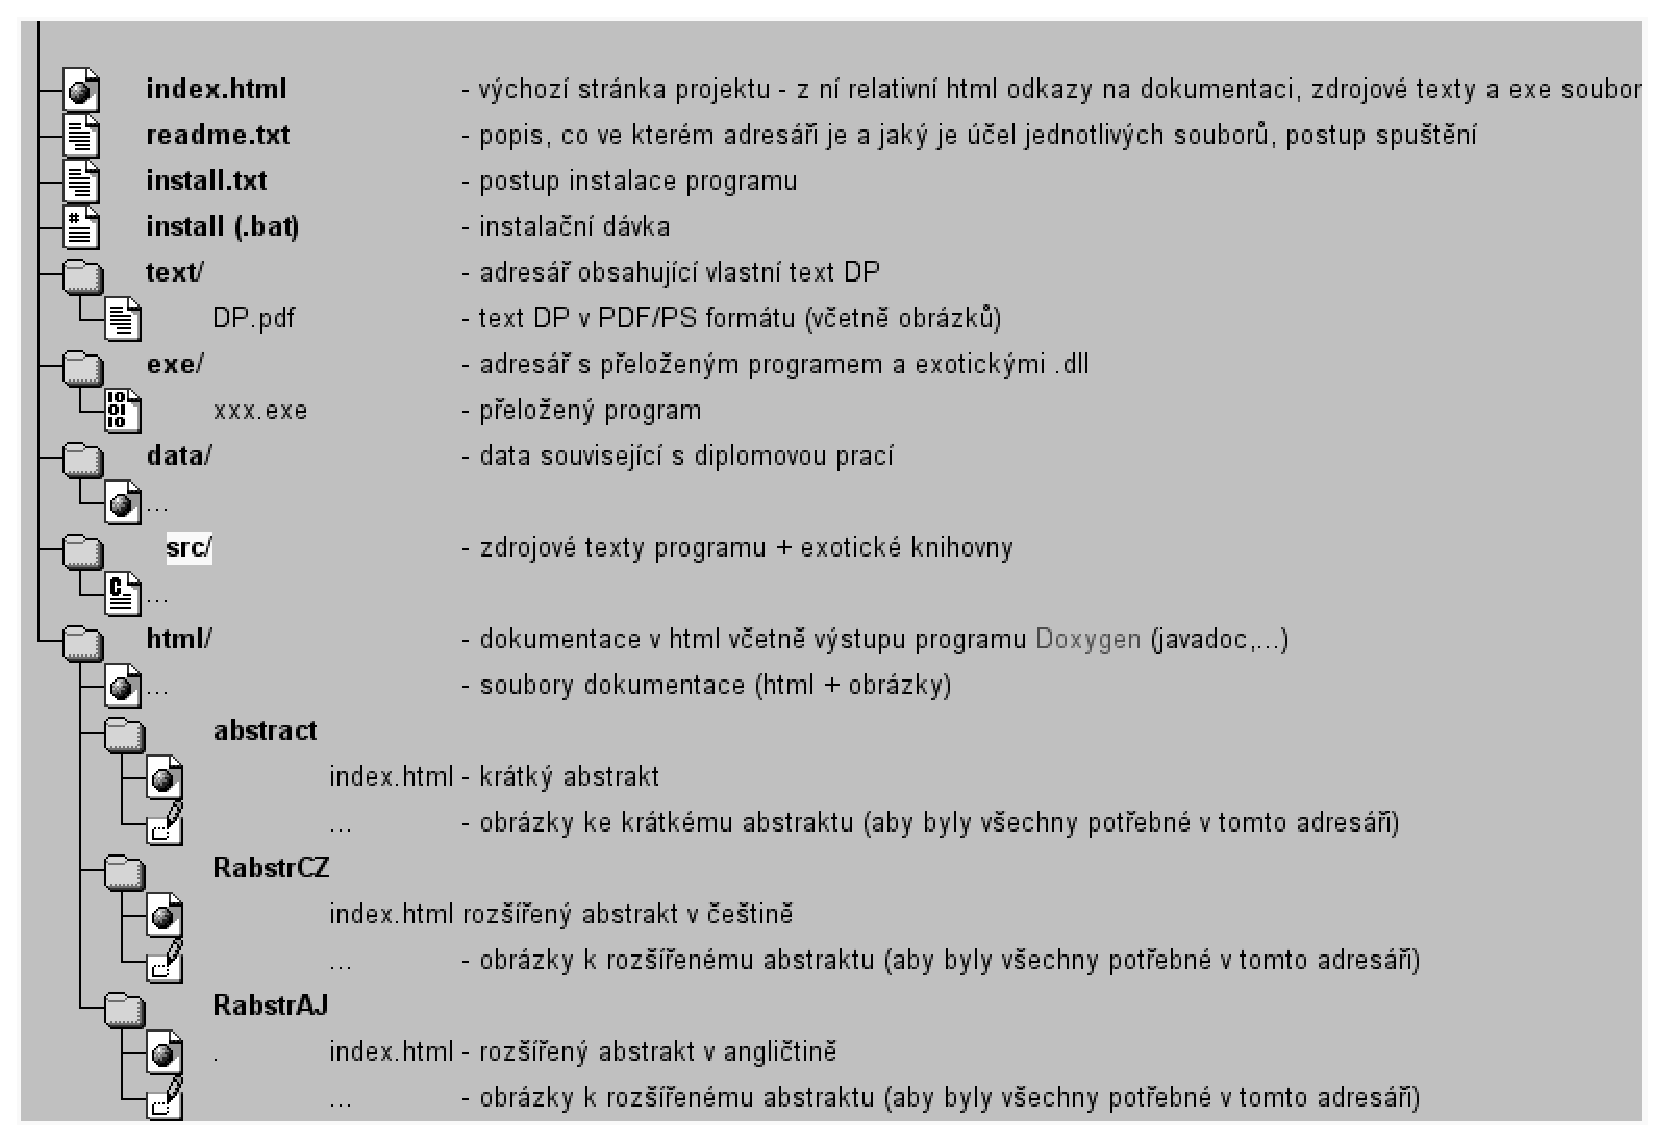
\includegraphics[width=14cm]{figures/seznamcd}
% \caption{Seznam přiloženého CD --- příklad}
% \label{fig:seznamcd}
% \end{center}
% \end{figure}
% 
% Na GNU/Linuxu si strukturu přiloženého CD můžete snadno vyrobit příkazem:\\ 
% \verb|$ tree . >tree.txt|\\
% Ve vzniklém souboru pak stačí pouze doplnit komentáře.
% 
% Z \textbf{README.TXT} (případne index.html apod.)  musí být rovněž zřejmé, jak programy instalovat, spouštět a jaké požadavky mají tyto programy na hardware.
% 
% Adresář \textbf{text}  musí obsahovat soubor s vlastním textem práce v PDF nebo PS formátu, který bude později použit pro prezentaci diplomové práce na WWW.

% Obsah přiloženého CD je zobrazený na obrázku \ref{fig:tree}.
% \begin{figure}[ht]
% \begin{center}
% 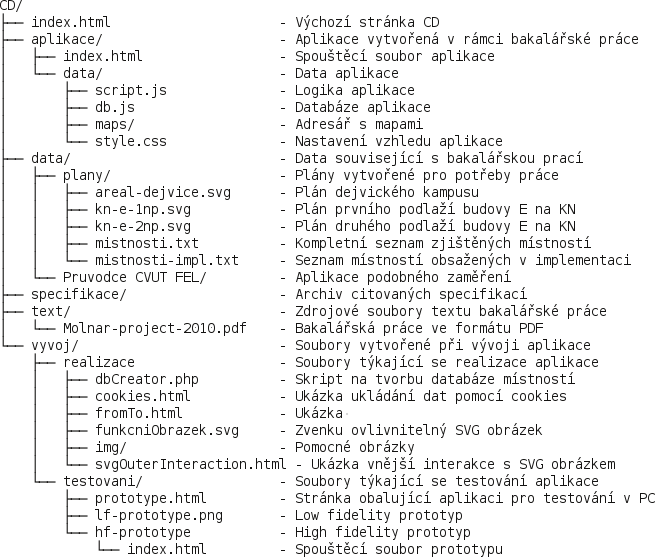
\includegraphics{figures/tree}
% % \caption{Struktura přiloženého CD}
% % \label{fig:tree}
% \end{center}
% \end{figure}

% $\vdash──$ \texttt{date-utils@1.2.10} -- popisek \\
% $\vdash─\top$ \texttt{express@2.5.6} \\
% $\mid \vdash─\top$ \texttt{connect@1.8.5} \\
% $\mid \mid └──$ \texttt{formidable@1.0.8} \\
% $\mid \vdash──$ \texttt{mime@1.2.4} \\
% $\mid \vdash──$ \texttt{mkdirp@0.0.7} \\
% $\mid └──$ \texttt{qs@0.4.1} \\
% $\vdash──$ \texttt{icalendar@0.4.1} \\
% $\vdash──$ \texttt{iconv@1.1.3} \\
% $\vdash─\top$ \texttt{jquery@1.6.3} \\
% $\mid \vdash──$ \texttt{htmlparser@1.7.4} \\
% $\mid └─\top$ \texttt{jsdom@0.2.10} \\
% $\mid   \vdash──$ \texttt{contextify@0.0.7} \\
% $\mid   \vdash──$ \texttt{cssom@0.2.2} \\
% $\mid   └──$ \texttt{request@2.9.100} \\
% $\vdash─\top$ \texttt{rdfstore@0.6.2} \\
% $\mid └──$ \texttt{mongodb@0.9.9-5} \\
% $└─\top$ \texttt{soap@0.1.2} \\
% $  \vdash──$ \texttt{node-expat@1.4.4/ \\
% $  └──$ \texttt{request@2.2.6} \\
% ├── date-utils@1.2.10 
% ├─┬ express@2.5.6 
% │ ├─┬ connect@1.8.5 
% │ │ └── formidable@1.0.8 
% │ ├── mime@1.2.4 
% │ ├── mkdirp@0.0.7 
% │ └── qs@0.4.1 
% ├── icalendar@0.4.1 
% ├── iconv@1.1.3 
% ├─┬ jquery@1.6.3 
% │ ├── htmlparser@1.7.4 
% │ └─┬ jsdom@0.2.10 
% │   ├── contextify@0.0.7 
% │   ├── cssom@0.2.2 
% │   └── request@2.9.100 
% ├─┬ rdfstore@0.6.2 
% │ └── mongodb@0.9.9-5 
% └─┬ soap@0.1.2 
%   ├── node-expat@1.4.4 
%   └── request@2.2.6 



\chapter{TODO}
\renewcommand*{\glspostdescription}{}
\printglossary[type=todo]
\noindent (Shodné položky jsou vynechány.)
% \listoffixmes

\end{document}
